%%% The main file. It contains definitions of basic parameters and includes all other parts.

%% Settings for single-side (simplex) printing
% Margins: left 40mm, right 25mm, top and bottom 25mm
% (but beware, LaTeX adds 1in implicitly)
\documentclass[12pt,a4paper]{report}
\setlength\textwidth{145mm}
\setlength\textheight{247mm}
\setlength\oddsidemargin{15mm}
\setlength\evensidemargin{15mm}
\setlength\topmargin{0mm}
\setlength\headsep{0mm}
\setlength\headheight{0mm}
% \openright makes the following text appear on a right-hand page
\let\openright=\clearpage

%% Settings for two-sided (duplex) printing
% \documentclass[12pt,a4paper,twoside,openright]{report}
% \setlength\textwidth{145mm}
% \setlength\textheight{247mm}
% \setlength\oddsidemargin{14.2mm}
% \setlength\evensidemargin{0mm}
% \setlength\topmargin{0mm}
% \setlength\headsep{0mm}
% \setlength\headheight{0mm}
% \let\openright=\cleardoublepage

%% Generate PDF/A-2u
\usepackage[a-2u]{pdfx}

%% Character encoding: usually latin2, cp1250 or utf8:
\usepackage[utf8]{inputenc}

%% Prefer Latin Modern fonts
\usepackage{lmodern}

%% Further useful packages (included in most LaTeX distributions)
\usepackage{amsmath}        % extensions for typesetting of math
\usepackage{amsfonts}       % math fonts
\usepackage{amsthm}         % theorems, definitions, etc.
\usepackage{bbding}         % various symbols (squares, asterisks, scissors, ...)
\usepackage{bm}             % boldface symbols (\bm)
\usepackage{graphicx}       % embedding of pictures
\usepackage{fancyvrb}       % improved verbatim environment
\usepackage{natbib}         % citation style AUTHOR (YEAR), or AUTHOR [NUMBER]
\usepackage[nottoc]{tocbibind} % makes sure that bibliography and the lists
			    % of figures/tables are included in the table
			    % of contents
\usepackage{dcolumn}        % improved alignment of table columns
\usepackage{booktabs}       % improved horizontal lines in tables
\usepackage{paralist}       % improved enumerate and itemize
\usepackage[usenames]{xcolor}  % typesetting in color


%%Added packages for particular thesis
\usepackage{tikz}
\usepackage{pgf}
\usepackage{amssymb}
%\usepackage[left]{lineno}
%\linenumbers
\usepackage{subfloat}
\usepackage{subfig}

\usetikzlibrary{arrows}

%%% Basic information on the thesis

% Thesis title in English (exactly as in the formal assignment)
\def\ThesisTitle{Enumeration of polyomino fillings}

% Author of the thesis
\def\ThesisAuthor{Bc. Mark Karpilovskij}

% Year when the thesis is submitted
\def\YearSubmitted{2018}

% Name of the department or institute, where the work was officially assigned
% (according to the Organizational Structure of MFF UK in English,
% or a full name of a department outside MFF)
\def\Department{Computer Science Institute of Charles University}

% Is it a department (katedra), or an institute (ústav)?
\def\DeptType{institute}

% Thesis supervisor: name, surname and titles
\def\Supervisor{doc. RNDr. Vít Jelínek, Ph.D.}

% Supervisor's department (again according to Organizational structure of MFF)
\def\SupervisorsDepartment{Computer Science Institute of Charles University}

% Study programme and specialization
\def\StudyProgramme{Computer Science}
\def\StudyBranch{Discrete Models and Algorithms}

% An optional dedication: you can thank whomever you wish (your supervisor,
% consultant, a person who lent the software, etc.)
\def\Dedication{%
I would like to express my sincere gratitude to my advisor, doc. Vít Jelínek, for guiding me through three years
of my university studies and sharing his great experience in mathematical research and writing.
}

% Abstract (recommended length around 80-200 words; this is not a copy of your thesis assignment!)
\def\Abstract{%
We prove two new results about 0-1-fillings of skew diagrams avoiding long increasing
and decreasing chains. In the first half of the thesis, we show that for a large class of skew diagrams, there
is a bijection between sparse fillings avoiding an increasing chain of fixed length
and sparse fillings avoiding a decreasing chain of the same length.
In the second half, we extend a known inequality between the number of sparse 0-1-fillings of skew diagrams avoiding an increasing chain of length 2
and a decreasing chain of length 2 to all 0-1-fillings.
}

% 3 to 5 keywords (recommended), each enclosed in curly braces
\def\Keywords{%
{polyomino} {filling} {skew diagram}
}

%% The hyperref package for clickable links in PDF and also for storing
%% metadata to PDF (including the table of contents).
%% Most settings are pre-set by the pdfx package.
%\hypersetup{unicode}
%\hypersetup{breaklinks=true}

% Definitions of macros (see description inside)
\include{macros}

% Title page and various mandatory informational pages
\begin{document}
\include{title}

%%% A page with automatically generated table of contents of the master thesis

\tableofcontents

%%% Each chapter is kept in a separate file
\chapter*{Introduction}
\addcontentsline{toc}{chapter}{Introduction}


A permutation $\pi$ is said to be \emph{contained} in a permutation $\sigma$,
if some rows and columns of the permutation matrix of $\sigma$ can be removed to obtain the permutation matrix of $\pi$,
otherwise $\sigma$ \emph{avoids} $\pi$. A set of permutations closed under containment is called a \emph{permutation class},
and it is a \emph{singleton class} if, in addition, it can be described as the set of all permutations avoiding a single permutation $\pi$.
Such a singleton class is denoted by $\text{Av}(\pi)$.
The study and enumeration of pattern-avoiding permutations and permutation classes has now been an active field for several decades.
One of the important concepts studied in this field is \emph{Wilf-equivalence}. Two permutation classes are \emph{Wilf-equivalent},
if for every positive integer $n$ they contain the same number of permutations of length $n$.

The search for new Wilf-equivalent classes has led to the investigation of a stronger kind of equivalence. Consider a Ferrers diagram
whose every cell is filled with a 0 or a 1 such that there is at most one 1 in every row and every column. Such a filling
of the Ferrers diagram is called \emph{sparse} and it \emph{contains}
a permutation $\sigma$, if some rows and columns of the Ferrers diagram can be removed to obtain the permutation matrix of $\sigma$,
otherwise it \emph{avoids} $\sigma$.
We then say that two singleton classes $\text{Av}(\pi)$ and $\text{Av}(\sigma)$ are \emph{shape-Wilf-equivalent} if for every
Ferrers diagram the number of sparse fillings avoiding $\pi$ is the same as the number of sparse fillings avoiding $\sigma$. 
The most notable example of shape-Wilf-equivalence was found by Backelin, West and Xin \cite{Backelin07}, who have
shown that for any $k$, the classes $\text{Av}(12\cdots k)$ and $\text{Av}(k(k-1)\cdots21)$ are shape-Wilf-equvalent.
Later, Krattenthaler \cite{Krattenthaler06} found a nice and simpler bijective proof of this result, and his work,
in return, was further generalized by Rubey \cite{Rubey11} who extended the bijection to more general diagrams.

In the present thesis, we prove two new results about 0-1-fillings of \emph{skew diagrams}, which are diagrams
obtained as difference of two Ferrers diagrams one of which contains the other. The thesis consists of three chapters.
In the first chapter, we introduce all of the necessary terminology and notation. In the second chapter,
we define a subclass of skew diagrams, the \emph{simple skew diagrams}, and 
make use of the approaches of Krattenthaler and Rubey to construct a bijection between sparse fillings
of a given simple skew diagram avoiding $12\cdots k$ and sparse fillings avoiding $k\cdots21$. In the final
chapter we generalise a result of Jelínek \cite{Jelinek08} and show that for every skew diagram,
there at least as many general fillings avoiding $12$ as there are fillings avoiding $21$.


\chapter{Preliminaries}

\section{Polyominoes}

A \emph{cell} is a unit square whose vertices lie on lattice points of the $\Z^2$ plane.
We then define a \emph{polyomino} as a finite set of cells. When referring to \emph{coordinates} of a cell,
we will use the $\Z^2$ coordinates of its bottom left corner.
A polyomino is \emph{convex} if for any two of its cells in the same row or column the polyomino also contains every cell in between.
Two columns of a polyomino are \emph{comparable} if the set of row coordinates of one column is contained in the set of row coordinates
of the other. We say that a polyomino is \emph{intersection-free} if any two of its columns are comparable. Note that this is equivalent
to having any two of its rows comparable. A \emph{moon polyomino} is a convex, intersection-free polyomino. A polyomino
is \emph{top-justified} if the top ends of all of its columns are in the same row and it is \emph{left-justified}
if the left ends of all of its rows are in the same column. Similarly we define a \emph{bottom-justified} or a
\emph{right-justified} polyomino.
A moon polyomino is a \emph{Ferrers diagram} if it is top-justified or bottom justified and in addition either left-justified or right-justified.

\begin{figure}[h]
\centering
\subfloat[][non-convex] {
\begin{tikzpicture}[line cap=round,line join=round,>=triangle 45,x=0.75cm,y=0.75cm]
\clip(1.56,0.49) rectangle (5.37,4.25);
\draw (2,4)-- (2,1);
\draw (2,1)-- (5,1);
\draw (5,1)-- (5,4);
\draw (5,4)-- (4,4);
\draw (4,4)-- (4,2);
\draw (4,2)-- (3,2);
\draw (3,2)-- (3,4);
\draw (3,4)-- (2,4);
\draw (2,3)-- (3,3);
\draw (2,2)-- (3,2);
\draw (4,2)-- (5,2);
\draw (4,2)-- (4,1);
\draw (3,2)-- (3,1);
\draw (4,3)-- (5,3);
\end{tikzpicture}
}
\subfloat[][convex, not \\ intersection-free] {
\begin{tikzpicture}[line cap=round,line join=round,>=triangle 45,x=0.75cm,y=0.75cm]
\clip(5.9,0.53) rectangle (9.1,4.25);
\draw (6,3)-- (6,1);
\draw (7,4)-- (7,1);
\draw (8,4)-- (8,1);
\draw (9,4)-- (9,2);
\draw (9,2)-- (6,2);
\draw (8,1)-- (6,1);
\draw (6,3)-- (9,3);
\draw (9,4)-- (7,4);
\end{tikzpicture}
}
\subfloat[][moon polyomino] {
\begin{tikzpicture}[line cap=round,line join=round,>=triangle 45,x=0.75cm,y=0.75cm]
\clip(9.52,0.36) rectangle (13.5,4.21);
\draw (10,3)-- (13,3);
\draw (12,4)-- (12,1);
\draw (11,4)-- (11,1);
\draw (10,2)-- (13,2);
\draw (13,2)-- (13,3);
\draw (12,4)-- (11,4);
\draw (10,3)-- (10,2);
\draw (11,1)-- (12,1);
\end{tikzpicture}
}
\subfloat[][bottom-justified moon polyomino] {
\centering
\begin{tikzpicture}[line cap=round,line join=round,>=triangle 45,x=0.75cm,y=0.75cm]
\clip(13.9,0.4) rectangle (17.56,4.25);
\draw (14,1)-- (17,1);
\draw (15,1)-- (15,4);
\draw (16,1)-- (16,4);
\draw (14,1)-- (14,3);
\draw (14,3)-- (16,3);
\draw (15,4)-- (16,4);
\draw (14,2)-- (17,2);
\draw (17,1)-- (17,2);
\end{tikzpicture}
}
\caption{Examples of polyominoes}
\label{figure_examples}
\end{figure}


A \emph{$NW$ Ferrers diagram} (standing for \emph{northwest}) is top-justified and left-justified.
A \emph{$SE$ Ferrers diagram} (standing for \emph{southeast}) is bottom-justified and right-justified.
We can represent both kinds of Ferrers diagrams by sequences of characters $R$ (meaning a step right) and $U$ (meaning step up),
describing the right-up border or the up-right border of $NW$ Ferrers diagrams or $SE$ Ferrers diagrams respectively.
For example, the $NW$ Ferrers diagram in Figure \ref{fig_nw_se}(a) is represented by the sequence 
\textit{RRURURRURUU}
and the $SE$ Ferrers diagram in Figure \ref{fig_nw_se}(b) is represented by the sequence 
\textit{URUUURRURR}. We call the sequences of characters $R$ and $U$ the \emph{$R$-$U$ sequences} and if a Ferrers diagram $F$
is represented by an $R$-$U$ sequence $w$, we say that $F$ \emph{is of type $w$}.

\begin{figure}[h]
\centering
\subfloat[][$NW$ Ferrers diagram] {
\begin{tikzpicture}[line cap=round,line join=round,>=triangle 45,x=1.0cm,y=1.0cm]
\clip(1.6,0) rectangle (8.24,6.22);
\draw (2,1)-- (2,6);
\draw (2,6)-- (8,6);
\draw (2,1)-- (4,1);
\draw (4,1)-- (4,2);
\draw (4,2)-- (5,2);
\draw (5,2)-- (5,3);
\draw (8,6)-- (8,4);
\draw (8,4)-- (7,4);
\draw (7,4)-- (7,3);
\draw (7,3)-- (5,3);

\draw (3,6)-- (3,1);
\draw (4,6)-- (4,2);
\draw (5,6)-- (5,3);
\draw (6,6)-- (6,3);
\draw (7,6)-- (7,4);
\draw (8,5)-- (2,5);
\draw (7,4)-- (2,4);
\draw (5,3)-- (2,3);
\draw (4,2)-- (2,2);

\end{tikzpicture}
}
\subfloat[][$SE$ Ferrers diagram] {
\begin{tikzpicture}[line cap=round,line join=round,>=triangle 45,x=1.0cm,y=1.0cm]
\clip(10.66,0) rectangle (16.45,6.9);
\draw (11,1)-- (16,1);
\draw (16,1)-- (16,6);
\draw (11,1)-- (11,2);
\draw (11,2)-- (12,2);
\draw (12,2)-- (12,5);
\draw (12,5)-- (14,5);
\draw (14,5)-- (14,6);
\draw (14,6)-- (16,6);
\draw (12,2)-- (16,2);
\draw (12,3)-- (16,3);
\draw (12,4)-- (16,4);
\draw (14,5)-- (16,5);
\draw (15,6)-- (15,1);
\draw (12,2)-- (12,1);
\draw (13,5)-- (13,1);
\draw (14,5)-- (14,1);
\end{tikzpicture}
}
\caption{Examples of Ferrers diagrams}
\label{fig_nw_se}
\end{figure}

Given a convex polyomino $P$, we define its \emph{height} $h(P)$ as the number of its nonempty rows. 
Similarly, we define its \emph{width} $w(P)$ as the number of nonempty columns of $P$.

Sometimes we will need to speak about the boundary of a convex polyomino, considered as a closed convex subset of the plane. We 
call the boundary of a convex polyomino $P$ the \emph{border} of $P$. If two adjacent sides of a cell of $\Z^2$ lie
on the border of $P$, the corner of the cell in which the two sides meet is a \emph{turn}
on the border. A line along the border between two adjacent turns of $M$ is a \emph{segment}. For example, the border
of the polyomino in Figure \ref{figure_examples}(b) consists of 8 turns and 8 segments.

\section{Partitions}
A \emph{partition} of length $n$ is a finite weakly decreasing sequence of positive integers $\lambda = (\lambda_1, \lambda_2, \ldots, \lambda_n)$. 
Each of the numbers $\lambda_i$ is called a \emph{part} of $\lambda$ and the \emph{size} of $\lambda$ is the sum of its parts.
Such a partition $\lambda$ also represents a $NW$ Ferrers diagram with column heights $\lambda_1, \ldots, \lambda_n$.
For example, the diagram in Figure \ref{fig_nw_se}(a) is represented by a partition $(5, 5, 4, 3, 3, 2)$. 
A partition $\mu = (\mu_1, \ldots, \mu_m)$ is \emph{contained} in $\lambda = (\lambda_1, \ldots, \lambda_n)$ if $m \leq n$
and $\mu_i \leq \lambda_i$ for $1 \leq i \leq m$.
The \emph{union} of partitions $\mu = (\mu_1, \ldots, \mu_m)$ and $\lambda = (\lambda_1, \ldots, \lambda_n)$ is
the partition $\nu = (\nu_1, \ldots, \nu_k)$ such that $k = \max(m, n)$ and $\nu_i = max(\mu_i, \lambda_i)$.
Finally, the \emph{transpose} of a partition $\lambda = (\lambda_1, \ldots, \lambda_n)$ is the partition
$\lambda^T = (\lambda^T_1, \ldots, \lambda^T_t)$ such that $t = \lambda_1$ and $\lambda^T_i$ is equal
to the number of parts of $\lambda$ greater than or equal to $i$. Notice that transposing
a partition is equivalent to reflecting the associated Ferrers diagram over the $y = x$ line.

\section{Skew diagrams}
A skew diagram is a $NW$ Ferrers diagram with a smaller $NW$ Ferrers diagram cut out of its north-west corner. This is represented
by a pair of partitions $(\lambda, \mu)$ such that $\mu$ is contained in $\lambda$.

\begin{figure}[h]
\centering
\begin{tikzpicture}[line cap=round,line join=round,>=triangle 45,x=1.0cm,y=1.0cm]
\clip(-4.15,-1.14) rectangle (1.12,3.15);
\draw (-4,-1)-- (-2,-1);
\draw (-2,-1)-- (-2,0);
\draw (-2,0)-- (0,0);
\draw (0,0)-- (0,2);
\draw (0,2)-- (1,2);
\draw (1,2)-- (1,3);
\draw (1,3)-- (-2,3);
\draw (-2,3)-- (-2,2);
\draw (-2,2)-- (-3,2);
\draw (-3,2)-- (-3,1);
\draw (-3,1)-- (-4,1);
\draw (-4,1)-- (-4,-1);
\draw [dash pattern=on 2pt off 2pt] (-4,1)-- (-4,3);
\draw [dash pattern=on 2pt off 2pt] (-4,3)-- (-2,3);
\draw (-2,3)-- (-2,0);
\draw (-1,3)-- (-1,0);
\draw (0,3)-- (0,2);
\draw (0,2)-- (-2,2);
\draw (0,1)-- (-3,1);
\draw (-2,0)-- (-4,0);
\draw [dash pattern=on 2pt off 2pt] (-3,2)-- (-3,3);
\draw [dash pattern=on 2pt off 2pt] (-3,2)-- (-4,2);
\draw (-3,1)-- (-3,-1);
\end{tikzpicture}
\caption{The skew diagram $((4,4,3,3,1),(2,1))$}
\end{figure}

Let $S$ be a skew diagram and let $C$ be one of its columns. We define the operation of \emph{deleting} the column $C$ from $S$
as removing the cells of $C$ and shifting all cells of $S$ right of $C$ one cell to the left. Similarly we define
the operation of deleting a row $R$ from $S$ as removing the cells of $R$ from $S$ and shifting all cells of $S$ below $R$
one cell upward.
A skew diagram $S$ is a \emph{subdiagram} of a skew diagram $T$ or is \emph{contained} in $T$ if $S$ can be created from $T$
by deleting some rows and columns. If $S$ is not containted in $T$, we say that $T$ \emph{avoids} $S$. Note that
both the class of skew diagrams and the class of Ferrers diagrams are closed under the operations of deleting a row or a column,
i.e. deleting a row or a column from a skew diagram always results in a skew diagram and in addition, if the diagram
is a Ferrers diagram, it remains a Ferrers diagram.

\begin{figure}[h]
\centering
\subfloat[][]{
\begin{tikzpicture}[line cap=round,line join=round,>=triangle 45,x=0.75cm,y=0.75cm]
\clip(-4.15,-1.14) rectangle (1.12,3.15);
\draw (-4,-1)-- (-2,-1);
\draw (-2,-1)-- (-2,0);
\draw (-2,0)-- (0,0);
\draw (0,0)-- (0,2);
\draw (0,2)-- (1,2);
\draw (1,2)-- (1,3);
\draw (1,3)-- (-2,3);
\draw (-2,3)-- (-2,2);
\draw (-2,2)-- (-3,2);
\draw (-3,2)-- (-3,1);
\draw (-3,1)-- (-4,1);
\draw (-4,1)-- (-4,-1);
\draw (-2,3)-- (-2,0);
\draw (-1,3)-- (-1,0);
\draw (0,3)-- (0,2);
\draw (0,2)-- (-2,2);
\draw (0,1)-- (-3,1);
\draw (-2,0)-- (-4,0);
\draw (-3,1)-- (-3,-1);
\draw [line width=1.6pt] (-3,-1) -- (-2,-1);
\draw [line width=1.6pt] (-2,-1) -- (-2,2);
\draw [line width=1.6pt] (-2,2) -- (-3,2);
\draw [line width=1.6pt] (-3,2) -- (-3,-1);
\end{tikzpicture}
}
\subfloat[][]{
\begin{tikzpicture}[line cap=round,line join=round,>=triangle 45,x=0.75cm,y=0.75cm]
\clip(-4.15,-1.14) rectangle (1.12,3.15);
\draw (-3,-1)-- (-2,-1);
\draw (-2,-1)-- (-2,0);
\draw (-2,0)-- (0,0);
\draw (0,0)-- (0,2);
\draw (0,2)-- (1,2);
\draw (1,2)-- (1,3);
\draw (1,3)-- (-2,3);
\draw (-2,3)-- (-2,2);
\draw (-3,1)-- (-3,1);
\draw (-3,1)-- (-3,-1);
\draw (-2,3)-- (-2,0);
\draw (-1,3)-- (-1,0);
\draw (0,3)-- (0,2);
\draw (0,2)-- (-2,2);
\draw (0,1)-- (-3,1);
\draw (-2,0)-- (-3,0);
\draw (-3,1)-- (-3,-1);
\end{tikzpicture}
}
\caption{Deleting a column from a skew diagram}
\label{figure_del_col}
\end{figure}

A skew diagram is clearly bounded by two paths leading from its lower left and to its upper right corner
and consisting only of steps up and to the right. We shall call them the \emph{upper border}
and the \emph{lower border} of the diagram.

For convenience, we will only consider \emph{connected} skew diagrams, which satisfy the additional condition that their
upper and lower borders only meet in the lower left and the upper right corner and nowhere in between. All of the presented 
results about connected skew diagrams can be extended to general skew diagrams without any effort.

\section{Fillings of polyominoes}

The main theme of this thesis is filling cells of polyominoes with integers and then counting fillings having certain properties.
A \emph{0-1-filling} of a polyomino is an assignment of either a 0 or a 1 to each cell of the polyomino.
A \emph{sparse filling} is a 0-1-filling, such that there is at most one 1 in each row and in each column. 
In figures, we will often represent 0's in such fillings by empty cells and 1's by crosses. In addition,
if a subset of a polyomino contains only 0's, we shall say that it is \emph{empty}, otherwise it is \emph{nonempty}.

\begin{figure}
\centering
\subfloat[][A sparse filling] {
\begin{tikzpicture}[line cap=round,line join=round,>=triangle 45,x=0.75cm,y=0.75cm]
\clip(-0.21,-1.19) rectangle (6.12,5.2);
\draw (1,4)-- (1,0);
\draw (1,0)-- (5,0);
\draw (5,0)-- (5,4);
\draw (5,4)-- (1,4);
\draw (2,0)-- (2,5);
\draw (3,0)-- (3,5);
\draw (4,0)-- (4,5);
\draw (2,5)-- (5,5);
\draw (5,5)-- (5,4);
\draw (3,0)-- (3,-1);
\draw (3,-1)-- (6,-1);
\draw (6,-1)-- (6,2);
\draw (6,2)-- (5,2);
\draw (5,1)-- (0,1);
\draw (5,2)-- (0,2);
\draw (5,3)-- (0,3);
\draw (0,1)-- (0,4);
\draw (0,4)-- (1,4);
\draw (4,0)-- (4,-1);
\draw (5,0)-- (5,-1);
\draw (5,0)-- (6,0);
\draw (5,1)-- (6,1);
\draw (0.5,3.5) node {$\times$};
\draw (2.5,2.5) node {$\times$};
\draw (4.5,1.5) node {$\times$};
\draw (1.5,0.5) node {$\times$};
\draw (3.5,4.5) node {$\times$};
\draw (5.5,-0.5) node {$\times$};
\end{tikzpicture}
}
\subfloat[][A non-sparse filling] {
\begin{tikzpicture}[line cap=round,line join=round,>=triangle 45,x=0.75cm,y=0.75cm]
\clip(-0.21,-1.19) rectangle (6.12,5.2);
\draw (1,4)-- (1,0);
\draw (1,0)-- (5,0);
\draw (5,0)-- (5,4);
\draw (5,4)-- (1,4);
\draw (2,0)-- (2,5);
\draw (3,0)-- (3,5);
\draw (4,0)-- (4,5);
\draw (2,5)-- (5,5);
\draw (5,5)-- (5,4);
\draw (3,0)-- (3,-1);
\draw (3,-1)-- (6,-1);
\draw (6,-1)-- (6,2);
\draw (6,2)-- (5,2);
\draw (5,1)-- (0,1);
\draw (5,2)-- (0,2);
\draw (5,3)-- (0,3);
\draw (0,1)-- (0,4);
\draw (0,4)-- (1,4);
\draw (4,0)-- (4,-1);
\draw (5,0)-- (5,-1);
\draw (5,0)-- (6,0);
\draw (5,1)-- (6,1);
\draw (1.5,0.5) node {$\times$};
\draw (1.5,2.5) node {$\times$};
\draw (2.5,2.5) node {$\times$};
\draw (3.5,2.5) node {$\times$};
\draw (3.5,3.5) node {$\times$};
\draw (4.5,4.5) node {$\times$};
\end{tikzpicture}
}
\caption{Examples of 0-1-fillings}
\label{figure_fillings}
\end{figure}

Let $P$ be a polyomino filled with a 0-1-filling and let $c_1, c_2, \ldots, c_l$ be $l$ of its cells filled with a 1.
These cells form a $NE$\emph{-chain (pronounced "northeast chain") of length} $l$ in $P$ if for $1 < i \leq l$ each $c_i$ is 
strictly northeast of $c_{i-1}$ and the smallest rectangle containing all $l$
cells is entirely contained in $P$. Similarly the cells form a $SE$\emph{-chain (pronounced "southeast chain") of length} $l$, if
for $1 < i \leq l$ each $c_i$ is strictly southeast of $c_{i-1}$ and again the smallest rectangle containing all the cells is entirely
contained in $P$. We then say that $P$ \emph{contains} a $NE$-chain (or $SE$-chain) of length $l$ if there is at least one 
occurence of such a chain in $P$. Otherwise we say that $P$ \emph{avoids} a $NE$-chain (or $SE$-chain) of length $l$.
For example, in Figure \ref{figure_chains}(a) the smallest rectangle containing the three nonzero entries are contained in the 
polyomino, so the 1's do form a $SE$-chain of length 3. However, in Figure \ref{figure_chains}(b) the northwest corner
of the smallest rectangle containing the four nonempty cells is not a part of the polyomino, so this is not a $NE$-chain of length 4.
However both the lower three 1's and the upper three 1's form a $NE$-chain of length 3.

\begin{figure}
\centering
\subfloat[][A $SE$-chain of length 3] {
\begin{tikzpicture}[line cap=round,line join=round,>=triangle 45,x=0.75cm,y=0.75cm]
\clip(-0.21,-1.19) rectangle (6.12,5.2);
\draw (1,4)-- (1,0);
\draw (1,0)-- (5,0);
\draw (5,0)-- (5,4);
\draw (5,4)-- (1,4);
\draw (2,0)-- (2,5);
\draw (3,0)-- (3,5);
\draw (4,0)-- (4,5);
\draw (2,5)-- (5,5);
\draw (5,5)-- (5,4);
\draw (3,0)-- (3,-1);
\draw (3,-1)-- (6,-1);
\draw (6,-1)-- (6,2);
\draw (6,2)-- (5,2);
\draw (5,1)-- (0,1);
\draw (5,2)-- (0,2);
\draw (5,3)-- (0,3);
\draw (0,1)-- (0,4);
\draw (0,4)-- (1,4);
\draw (4,0)-- (4,-1);
\draw (5,0)-- (5,-1);
\draw (5,0)-- (6,0);
\draw (5,1)-- (6,1);
\draw (0.5,3.5) node {$\times$};
\draw (2.5,2.5) node {$\times$};
\draw (4.5,1.5) node {$\times$};
\end{tikzpicture}
}
\subfloat[][Not a $NE$-chain of length 4] {
\begin{tikzpicture}[line cap=round,line join=round,>=triangle 45,x=0.75cm,y=0.75cm]
\clip(-0.21,-1.19) rectangle (6.12,5.2);
\draw (1,4)-- (1,0);
\draw (1,0)-- (5,0);
\draw (5,0)-- (5,4);
\draw (5,4)-- (1,4);
\draw (2,0)-- (2,5);
\draw (3,0)-- (3,5);
\draw (4,0)-- (4,5);
\draw (2,5)-- (5,5);
\draw (5,5)-- (5,4);
\draw (3,0)-- (3,-1);
\draw (3,-1)-- (6,-1);
\draw (6,-1)-- (6,2);
\draw (6,2)-- (5,2);
\draw (5,1)-- (0,1);
\draw (5,2)-- (0,2);
\draw (5,3)-- (0,3);
\draw (0,1)-- (0,4);
\draw (0,4)-- (1,4);
\draw (4,0)-- (4,-1);
\draw (5,0)-- (5,-1);
\draw (5,0)-- (6,0);
\draw (5,1)-- (6,1);
\draw (1.5,0.5) node {$\times$};
\draw (2.5,2.5) node {$\times$};
\draw (3.5,3.5) node {$\times$};
\draw (4.5,4.5) node {$\times$};
\end{tikzpicture}
}
\caption{Examples of chains in a polyomino with a 0-1-filling}
\label{figure_chains}
\end{figure}

In the following chapter we deal with sparse fillings of skew diagrams avoiding long $NE$-chains and $SE$-chains. To describe
the sets of fillings in question easily, we will use the notation introduced by Rubey \cite{Rubey11}.

\begin{defn}[{\cite[Definition 5.2]{Rubey11}}]\label{def_rubey}
Let $P$ be a moon polyomino or a connected skew diagram, 
$l$ a positive integer and $\bm{r}$, $\bm{c}$ sequences of 0's and 1's of lengths $h(P)$ and $w(P)$ respectively.
Then $\F^{NE}(P, l, \bm{r}, \bm{c})$ is the set of all sparse fillings of $P$ such that
\begin{itemize}
\item there is a 1 in the $i$-th row of $P$ if and only if $r_i = 1$,
\item there is a 1 in the $i$-th column of $P$ if and only if $c_i = 1$,
\item the length of the longest $NE$-chain in the filling is equal to $l$.
\end{itemize}
\end{defn}

Similarly we define $\F^{SE}(P, l, \bm{r}, \bm{c})$ as the set of all sparse fillings of $P$ with the length of the longest $SE$-chain
equal to $l$ and having 1's exactly in the rows and columns prescribed by $\bm{r}$ and $\bm{c}$. Note that since we are dealing with sparse fillings,
the number of nonempty rows and columns prescribed by $\bm{r}$ and $\bm{c}$ must be the same for any fillings to exist.


\chapter{A bijection between fillings of special skew diagrams}

\section{Main result}

Let $S^{forb}$ be the forbidden skew diagram $((3,3,2),(1))$.

\begin{figure}[h]
\centering
\begin{tikzpicture}[line cap=round,line join=round,>=triangle 45,x=0.75cm,y=0.75cm]
\clip(5.9,0.53) rectangle (9.1,4.25);
\draw (6,3)-- (6,1);
\draw (7,4)-- (7,1);
\draw (8,4)-- (8,1);
\draw (9,4)-- (9,2);
\draw (9,2)-- (6,2);
\draw (8,1)-- (6,1);
\draw (6,3)-- (9,3);
\draw (9,4)-- (7,4);
\end{tikzpicture}
\caption{$S^{forb}$}
\end{figure}

\begin{lemma} \label{lemma_forb_rec}
A skew diagram $S$ avoids $S^{forb}$ if and only if for every cell $c$ of $S$ at least one
of the following conditions is satisfied:
\begin{itemize}
\item
either the set
of cells of $S$ to the left and above $c$ (including the cells in the same row or column as $c$)
forms a rectangle, or 
\item the set of cells of $S$ to the right and below of $c$ (including the cells in the same row or column
as $c$) forms a rectangle.
\end{itemize}
\end{lemma}
\begin{proof}
If $S$ does contain $S^{forb}$, then the cell that represents the middle cell of an occurence of $S^{forb}$ violates both conditions.
On the other hand, if a cell $c$ of $S$ violates both conditions, we find an occurence of $S^{forb}$ in $S$ with this cell as its middle cell.
Let $A$ be the maximal rectangle contained in $S$ which has $c$ as its northeast corner and let $B$ be the maximal rectangle contained
in $S$ which has $c$ as its southwest corner. Then the 7 cells in the corners of these two rectangles form an occurence of $S^{forb}$.
\end{proof}

We can now formulate the main result of this chapter.

\begin{thm} \label{thm_main}
Let $S$ be a skew diagram avoiding $S^{forb}$, let $l \geq 1$ be an integer and let $\bm{r}$ and $\bm{c}$ be sequences of 0's
and 1's of lengths $w(S)$ and $h(S)$ respectively. Then there is a bijection between 
the sets $\F^{NE}(S, l, \bm{r}, \bm{c})$ and $\F^{SE}(S, l, \bm{r}, \bm{c})$.
\end{thm}

To prove this theorem, we will utilize other known bijection theorems on Ferrers diagrams and moon polyominoes
described in sections \ref{sec3} and \ref{sec4}, but first,
we will prove a useful equivalent characterization of skew diagrams avoiding $S^{forb}$.

\section{Simple skew diagrams}

Let $S$ be a skew diagram and let a vertical line leading between two adjacent columns of $S$ divide it into two skew diagrams $S_1$ and
$S_2$. Then we say that $S$ is a \emph{vertical concatenation} of $S_1$ and $S_2$ and we write $S = S_1 |^v S_2$. Similarly we define
\emph{horizontal concatenation} and write $T = T_1 |^h T_2$. Note that there are mutiple ways how to concatenate two skew diagrams.

We say that $S$ is a \emph{simple skew diagram} if it can be written as 

$$S = F_1 |^v G_1 |^h F_2 |^v \cdots |^h F_n |^v G_n,$$

where all $F_i$ are $NW$ Ferrers diagrams, all $G_i$ are $SE$ Ferrers diagrams and all $F_i$ and $G_i$ are nonempty with the possible
exception of $G_n$. We call this representation of $S$ the \emph{simple representation}.

\begin{figure}[h]
\centering
\begin{tikzpicture}[line cap=round,line join=round,>=triangle 45,x=0.75cm,y=0.75cm]
\clip(-4.25,-4.33) rectangle (6.19,4.2);
\draw (-4,-4)-- (-4,0);
\draw (-4,0)-- (0,0);
\draw (0,0)-- (0,-2);
\draw (0,-2)-- (-1,-2);
\draw (-1,-2)-- (-1,-3);
\draw (-1,-3)-- (-2,-3);
\draw (-2,-3)-- (-2,-4);
\draw (-2,-4)-- (-4,-4);
\draw (0,0)-- (0,1);
\draw (0,1)-- (2,1);
\draw (2,1)-- (2,2);
\draw (0,-1)-- (4,-1);
\draw (2,2)-- (4,2);
\draw (4,2)-- (4,-1);
\draw (-2.8,-1.35) node[anchor=north west] {$F_1$};
\draw (1.64,0.42) node[anchor=north west] {$G_1$};
\draw (2,2)-- (5,2);
\draw (3,2)-- (3,4);
\draw (3,4)-- (6,4);
\draw (6,4)-- (6,3);
\draw (6,3)-- (5,3);
\draw (5,3)-- (5,2);
\draw (3.5,3.35) node[anchor=north west] {$F_2$};
\end{tikzpicture}
\caption{A simple skew skew diagram}
\end{figure}

The key lemma follows.

\begin{lemma} \label{lemma_key}
A skew diagram is simple if and only if it does not contain $S^{forb}$.
\end{lemma}
\begin{proof}
In a simple skew diagram $S$ every cell is in either a $NW$ Ferrers subdiagram or a $SE$ Ferrers subdiagram and thus satisfies
at least one of the conditions
of Lemma \ref{lemma_forb_rec}. Therefore $S$ avoids $S^{forb}$. 

We now prove that every skew diagram avoiding $S^{forb}$ is simple by induction on the number of turns on the upper border of a skew diagram. 
If there is only one turn on the upper border of a skew diagram, then it is necessarily a $NW$ Ferrers diagram and there is nothing to prove.
Let $S$ be a skew diagram whose upper border has at least two turns.

Let $u_1$ and $r_1$ be the first two segments of the upper border of $S$, starting from the lower left corner, with $u_1$ going up
and $r_1$ going to the right. Together with the corresponding part of the lower border they bound a $NW$ Ferrers diagram
$F$ which can be separated by a vertical line $v$ from the rest of $S$, as we can see in Figure \ref{figure_key_lemma}.

Next, consider the cell $c$ attached to the upper right corner of $F$ as indicated in Figure \ref{figure_key_lemma}.
Since $S$ avoids $S^{forb}$ and the upper right corner of $c$ is a turn of the border of $S$, we get by Lemma \ref{lemma_forb_rec}
that the part of $S$ to the left and below of $c$ must form a rectangle, bounded from below by the lower border segment $r_2$
and from the right by the lower border segment $u_2$. These two segments of the lower border, together with
the corresponding part of the upper border of $S$ bound a $SE$ Ferrers diagram $G$, which can again be separated from the 
rest of $S$ by a horizontal line $h$.

Finally, let $S'$ be the part of $S$ above the line $h$. Then $S'$ is a skew diagram which definitely has fewer turns
on its upper border than $S$, so the induction applies and we get that $S'$ can be written as

$$S' = F_1 |^v G_1 |^h F_2 |^v \cdots |^h F_n |^v G_n,$$

where $F_1, \ldots, F_n$ are nonempty $NW$ Ferrers diagrams and $G_1, \ldots, G_n$ are $SE$ Ferrers diagrams. Together
with the constructed diagrams $F$ and $G$ we get that

$$S = F |^v G |^h F_1 |^v G_1 |^h F_2 |^v \cdots |^h F_n |^v G_n,$$

and thus $S$ is simple.

\begin{figure}[h]
\centering
\begin{tikzpicture}[line cap=round,line join=round,>=triangle 45,x=1.0cm,y=1.0cm]
\clip(1.57,2) rectangle (15.59,10.27);
\fill[fill=black,fill opacity=0.1] (7,7) -- (7,6.68) -- (7.32,6.68) -- (7.32,7) -- cycle;
\draw (3,3)-- (3,7);
\draw (3,7)-- (7,7);
\draw (7,10)-- (7,1);
\draw [shift={(3.34,6.88)},dash pattern=on 2pt off 2pt]  plot[domain=4.62:5.93,variable=\t]({1*3.89*cos(\t r)+0*3.89*sin(\t r)},{0*3.89*cos(\t r)+1*3.89*sin(\t r)});
\draw (7,6)-- (10,6);
\draw (10,6)-- (10,9);
\draw (4,9)-- (15,9);
\draw [shift={(9.6,6.48)},dash pattern=on 2pt off 2pt]  plot[domain=1.88:2.94,variable=\t]({1*2.65*cos(\t r)+0*2.65*sin(\t r)},{0*2.65*cos(\t r)+1*2.65*sin(\t r)});
\draw (7,7)-- (7,6.68);
\draw (7,6.68)-- (7.32,6.68);
\draw (7.32,6.68)-- (7.32,7);
\draw (7.32,7)-- (7,7);
\begin{scriptsize}
\draw[color=black] (2.75,5.11) node {\normalsize $u_1$};
\draw[color=black] (4.85,7.29) node {\normalsize $r_1$};
\draw[color=black] (7.14,4.38) node {\normalsize $v$};
\draw[color=black] (8.56,5.86) node {\normalsize $r_2$};
\draw[color=black] (10.19,7.62) node {\normalsize $u_2$};
\draw[color=black] (10.8,9.23) node {\normalsize $h$};
\draw[color=black] (7.74,6.72) node {\normalsize $c$};
\draw[color=black] (4.8,5.2) node {\large $F$};
\draw[color=black] (8.5,7.5) node {\large $G$};
\end{scriptsize}
\end{tikzpicture}
\caption{}
\label{figure_key_lemma}
\end{figure}
\end{proof}

\section{The bijection on Ferrers diagrams} \label{sec3}
Krattenthaler \cite{Krattenthaler06} proved Theorem \ref{thm_main} for the special case of Ferrers diagrams using the growth diagram
construction developed by Britz and Fomin \cite{Fomin01}. We briefly introduce growth diagrams
and reformulate the results of this approach in our setting. For convenience, we will describe the construction for $NW$
Ferrers diagrams only, however, the modification for $SE$ diagrams is obvious and we shall use it without stating it properly.

\begin{figure}[h]
\centering
\begin{tikzpicture}[line cap=round,line join=round,>=triangle 45,x=1.0cm,y=1.0cm]
\clip(0,0) rectangle (3,3);
\draw (1,1)--(1,2);
\draw (1,2)--(2,2);
\draw (2,2)--(2,1);
\draw (2,1)--(1,1);
\draw (0.8, 0.8) node {$\nu$};
\draw (0.8, 2.2) node {$\lambda$};
\draw (2.2, 2.2) node {$\mu$};
\draw (2.2, 0.8) node {$\rho$};
\end{tikzpicture}
\caption{A cell of a growth diagram}
\label{figure_growth_cell}
\end{figure}

Let $F$ be a Ferrers diagram filled with a sparse filling. 
We will inductively label every corner of every cell of $F$ by a partition, obtaining a \emph{growth diagram}.
We start by labeling the corners on the left and upper borders by the empty partition $\emptyset$. If a cell
already has all corners except the lower-right corner labeled by partitions $\lambda$, $\mu$, and $\nu$ as in Figure \ref{figure_growth_cell},
we construct the remaining partition $\rho$ by the following \emph{forward local} rules:
\begin{itemize}
\item [(F1)] If the cell does not contain a 1 and $\lambda = \mu = \nu$, then $\rho = \lambda$.
\item [(F2)] If the cell does not contain a 1 and $\mu \neq \nu$, then $\rho = \mu \cup \nu$.
\item [(F3)] If the cell does not contain a 1, $\lambda \subsetneq \mu = \nu$ and $\lambda$ and $\mu$ differ in their $i$-th part,
then we obtain $\rho$ by increasing the $i+1$-th part of $\mu$ by 1.
\item [(F4)] If the cell contains a 1, then necessarily $\lambda = \nu = \mu$ and we obtain $\rho$ by increasing the first
part of $\lambda$ by 1. 
\end{itemize}

Note that the equality of partitions in (F4) is implied by the fact that there is no 1 in the row of cells to the left or 
in the column of cells above the considered cell.

\begin{figure}
\centering
\begin{tikzpicture}[line cap=round,line join=round,>=triangle 45,x=1.0cm,y=1.0cm]
\clip(0,0) rectangle (6,6);

\draw (1,1)--(1,5);
\draw (2,1)--(2,5);
\draw (3,1)--(3,5);
\draw (4,2)--(4,5);
\draw (5,3)--(5,5);


\draw (1,1)--(3,1);
\draw (1,2)--(4,2);
\draw (1,3)--(5,3);
\draw (1,4)--(5,4);
\draw (1,5)--(5,5);

\draw (1.5, 3.5) node {\large $\times$};
\draw (2.5, 2.5) node {\large $\times$};
\draw (3.5, 4.5) node {\large $\times$};

\draw (1.2, 1.2) node {\footnotesize $\emptyset$};
\draw (1.2, 2.2) node {\footnotesize $\emptyset$};
\draw (1.2, 3.2) node {\footnotesize $\emptyset$};
\draw (1.2, 4.2) node {\footnotesize $\emptyset$};
\draw (1.2, 5.2) node {\footnotesize $\emptyset$};
\draw (2.2, 1.2) node {\footnotesize $1$};
\draw (2.2, 2.2) node {\footnotesize $1$};
\draw (2.2, 3.2) node {\footnotesize $1$};
\draw (2.2, 4.2) node {\footnotesize $\emptyset$};
\draw (2.2, 5.2) node {\footnotesize $\emptyset$};
\draw (3.2, 1.2) node {\footnotesize $2$};
\draw (3.2, 2.2) node {\footnotesize $2$};
\draw (3.2, 3.2) node {\footnotesize $1$};
\draw (3.2, 4.2) node {\footnotesize $\emptyset$};
\draw (3.2, 5.2) node {\footnotesize $\emptyset$};
\draw (4.2, 2.2) node {\footnotesize $21$};
\draw (4.2, 3.2) node {\footnotesize $11$};
\draw (4.2, 4.2) node {\footnotesize $1$};
\draw (4.2, 5.2) node {\footnotesize $\emptyset$};
\draw (5.2, 3.2) node {\footnotesize $11$};
\draw (5.2, 4.2) node {\footnotesize $1$};
\draw (5.2, 5.2) node {\footnotesize $\emptyset$};



\end{tikzpicture}
\caption{An example of a growth diagram}
\label{figure_growth_diagram}
\end{figure}


Let $w=w_1w_2\cdots w_k$ be an $R$-$U$ sequence. 
An \emph{oscillating tableau of type $w$ and shape $\emptyset/\emptyset$} 
is a sequence of partitions $(\lambda^0, \lambda^1, \ldots, \lambda^k)$ with the following properties:
\begin{itemize}
\item $\lambda^0 = \lambda^k = \emptyset$
\item For $1 \leq i \leq k$, the sizes of $\lambda^{i-1}$ and $\lambda^i$ differ by at most 1.
\item If $w_i = R$, then $\lambda^{i-1} \subseteq \lambda^i$.
\item If $w_i = U$, then $\lambda^{i-1} \supseteq \lambda^i$.
\end{itemize}

Remarkably, both the filling and the entire growth diagram of a Ferrers diagram of type $w$ can be reconstructed from
the sequence of partitions labeling the corners of its south-east border, which clearly is an oscillating tableau
of type $w$ and shape $\emptyset/\emptyset$. For more details we refer the reader to \cite[Section 2]{Krattenthaler06}.
The main consequence of this construction is the following theorem.

\begin{thm}[{\cite[Theorem 1]{Krattenthaler06}}] \label{thm_krat_1}
Let $F$ be a $NW$ Ferrers diagram of type $w = w_1w_2\ldots w_k$. The mapping, which to each sparse filling of $F$
assigns the oscillating tableau $(\emptyset = \lambda^0, \lambda^1, \ldots, \lambda^k = \emptyset)$
constructed as shown above, is a bijection between the set of all sparse fillings of $F$
and the set of all oscillating tableaux of type $w$ and shape $\emptyset/\emptyset$. In addition, this mapping has the following properties:
\begin{itemize}
\item $\lambda^{i-1} \subsetneq \lambda^i$ if and only if there is a $1$ in the column above the corners labeled by $\lambda^{i-1}$
and $\lambda^{i}$.
\item $\lambda^{i} \subsetneq \lambda^{i-1}$ if and only if there is a $1$ in the row to the left of the corners labeled by $\lambda^{i-1}$
and $\lambda^{i}$.
\end{itemize}
\end{thm}

For example, the filling of the Ferrers diagram in Figure \ref{figure_growth_diagram} is mapped to the oscillating tableau
$(\emptyset, 1, 2, 2, 21, 11, 11, 1, \emptyset)$. 

The very useful fact about growth diagrams 
is that the lengths of both longest $NE$-chains and $SE$-chains in a Ferrers
diagram can be deduced from partitions labeling the corners.

\begin{thm}[{\cite[Theorem 2]{Krattenthaler06}}] \label{thm_greene}
Let $F$ be a Ferrers diagram with a sparse filling and a growth diagram constructed accordingly and let $\lambda = (\lambda_1, \ldots, \lambda_k)$
be a partition labeling the southwest corner of a cell $c$. 
Let $R$ be the maximal rectangle contained in $F$ with the cell $c$ in its southwest corner.
Then the longest $NE$-chain contained in $R$ has length $k$ and the longest $SE$-chain contained in $R$ has length $\lambda_1$.
\end{thm}

Using growth diagrams and the theorems above it is now easy to prove Theorem \ref{thm_main} for Ferrers diagrams.

\begin{thm}[{\cite[Theorem 3]{Krattenthaler06}}] \label{thm_krat_3}
Let $F$ be a Ferrers diagram and $l \geq 1$ an integer. Let $\bm{r}$ and $\bm{c}$ be sequences of 0's and 1's
of length $w(F)$ and $h(F)$ respectively. 
Then there is a bijection between the sets $\F^{NE}(F, l, \bm{r}, \bm{c})$ and $\F^{SE}(F, l, \bm{r}, \bm{c})$.
\end{thm}
\begin{proof}
For given sequences $\bm{r}$ and $\bm{c}$ let $F'$ be the diagram obtained from $F$ by deleting the rows
with a 0 entry in $\bm{r}$ and columns with a 0 entry in $\bm{c}$. Since the deleted rows and columns
are always empty in the considered fillings, it is enough to construct a bijection
between the sets $\F^{NE}(F',l,\bm{1},\bm{1})$ and $\F^{SE}(F',l,\bm{1},\bm{1})$ where $\bm{1}$ is a sequence of only 1's
and this bijection is trivially extended to the sets in question.

Choose a filling of $F'$ from $\F^{NE}(F',l,\bm{1},\bm{1})$. The Theorem \ref{thm_krat_1} assigns to this filling
an oscillating tableau $(\emptyset = \lambda^0, \lambda^1, \ldots, \lambda^k = \emptyset)$ and by Theorem \ref{thm_greene}
every partition $\lambda^i$ has at most $l$ parts with equality occuring at least once. Now consider
the oscillating tableau $(\emptyset = (\lambda^0)^T, (\lambda^1)^T, \ldots, (\lambda^k)^T = \emptyset)$
obtained by transposing every partition of the original tableau. We use the Theorem \ref{thm_krat_1} again
to assign a sparse filling of $F'$ to the transposed tableau. Since the transposition does not change the size
of a partition, it is true that $(\lambda^{i-1})^T$ and $(\lambda^{i})^T$ differ by 1 in size for each $1 \leq i \leq k$
and therefore the obtained filling of $F'$ contains a 1 in each row and each column. In addition, each $(\lambda^i)^T$
satisfies $(\lambda^i)^T_1 \leq l$ with equality occuring at least once and so by Theorem \ref{thm_greene} the
length of the longest $SE$-chain in $F'$ is equal to $l$. Therefore, the obtained filling is in $\F^{SE}(F', l, \bm{1}, \bm{1})$.
\end{proof}

\section{A bijection on moon polyominoes} \label{sec4}

In his work, Rubey \cite{Rubey11} proves more general bijective results about fillings of moon polyominoes. In particular,
he shows that permuting the columns of a moon polyomino in any way such that it remains a moon polyomino does not change
the number of 0-1 fillings having a fixed length of the longest $NE$-chain and prescribed number of 1's in each row.
Here we formulate a part of his results which will be useful in our efforts. 

Given a finite sequence $s = (s_1, s_2, \ldots, s_n)$ and a permutation $\sigma$ of length $n$,
we denote by $\sigma s$ the sequence $(s_{\sigma(1)}, s_{\sigma(2)}, \ldots, s_{\sigma(n)})$. In addition,
given a moon polyomino $M$ and a permutation $\pi$ of length $w(M)$, we denote by $\sigma M$ the polyomino created by
permuting the columns of $M$ according to $\pi$. We will also need a stronger version of Definition \ref{def_rubey}.

\begin{defn}[{\cite[Definition 5.2]{Rubey11}}]\label{def_strong_rubey}
Let $M$ be a moon polyomino, $\bm{r}$, $\bm{c}$ sequences of 0's and 1's of lengths $h(M)$ and $w(M)$ respectively
and $\Lambda$ a mapping which assigns to every maximal rectangle $R$ in $M$ a positive integer $\Lambda(R)$.
Then $\F^{NE}(M, \Lambda, \bm{r}, \bm{c})$ is the set of all sparse fillings of $P$ such that
\begin{itemize}
\item there is a 1 in the $i$-th row of $P$ if and only if $r_i = 1$,
\item there is a 1 in the $i$-th column of $P$ if and only if $c_i = 1$,
\item for every maximal rectangle $R$ the length of the longest $NE$-chain in the filling of $R$ is equal to $\Lambda(R)$.
\end{itemize}
\end{defn}

Note that in a moon polyomino, every maximal rectangle is uniquely determined by its height and width. 
Indeed, consider two maximal rectangles of the same height in a moon polyomino $M$. Since the columns of the two rectangles
are comparable, they must in fact span the same rows, and since $M$ is convex, they must be contained in each other and thus
be identical.

\begin{thm}[{\cite[Theorem 5.3]{Rubey11}}]\label{thm_rubey}
Let $M$ be a moon polyomino and $R$ be a maximal rectangle in $M$ such that the column of $M$ containing 
the leftmost column $C$ of $R$ has the same height as $C$. Let $\sigma$ be the permutation of columns of $M$
which moves the column $C$ to the right end of $R$ and shifts the other columns intersecting $R$ one spot to the left.
Then the sets of maximal rectangles of $M$ and $\sigma M$ coincide and 
for any $\Lambda$, $\bm{r}$ and $\bm{c}$ there is a bijective map which maps every filling in $\F^{NE}(M, \Lambda, \bm{r}, \bm{c})$ to a 
filling in $\F^{NE}(\sigma M, \Lambda, \bm{r}, \bm{\sigma c})$.
\end{thm}

\begin{figure}
\centering
\subfloat[][$M$]{
\begin{tikzpicture}[line cap=round,line join=round,>=triangle 45,x=0.75cm,y=0.75cm]
\clip(0.86,1.79) rectangle (9.18,9.16);
\draw (3,8)-- (3,4);
\draw (3,4)-- (8,4);
\draw (8,4)-- (8,8);
\draw (8,8)-- (3,8);
\draw (4,8)-- (4,4);
\draw (5,8)-- (5,4);
\draw (6,8)-- (6,4);
\draw (7,8)-- (7,4);
\draw (4,7)-- (8,7);
\draw (4,6)-- (8,6);
\draw (4,5)-- (8,5);
\draw (3,7)-- (1,7);
\draw (1,7)-- (1,6);
\draw (1,6)-- (3,6);
\draw (2,7)-- (2,4);
\draw (2,4)-- (3,4);
\draw (2,5)-- (3,5);
\draw (4,4)-- (4,3);
\draw (4,3)-- (8,3);
\draw (8,3)-- (8,4);
\draw (7,3)-- (7,2);
\draw (7,2)-- (4,2);
\draw (4,2)-- (4,3);
\draw (5,8)-- (5,9);
\draw (5,9)-- (7,9);
\draw (7,9)-- (7,8);
\draw (6,8)-- (6,9);
\draw (8,7)-- (9,7);
\draw (9,7)-- (9,4);
\draw (9,4)-- (8,4);
\draw (5,4)-- (5,2);
\draw (6,4)-- (6,2);
\draw (8,6)-- (9,6);
\draw (8,5)-- (9,5);
\draw (7,4)-- (7,3);
\draw (3.5, 6) node {$C$};
\draw [line width=1.6pt] (3,4) -- (3,8);
\draw [line width=1.6pt] (8,8) -- (3,8);
\draw [line width=1.6pt] (8,8) -- (8,4);
\draw [line width=1.6pt] (3,4) -- (8,4);
\end{tikzpicture}
}
\subfloat[][$\sigma M$]{
\begin{tikzpicture}[line cap=round,line join=round,>=triangle 45,x=0.75cm,y=0.75cm]
\clip(2.74,0.77) rectangle (11.15,8.17);
\draw (5,7)-- (5,3);
\draw (5,3)-- (10,3);
\draw (10,3)-- (10,7);
\draw (10,7)-- (5,7);
\draw (6,7)-- (6,3);
\draw (7,7)-- (7,3);
\draw (8,7)-- (8,3);
\draw (9,7)-- (9,3);
\draw (5,6)-- (3,6);
\draw (3,6)-- (3,5);
\draw (3,5)-- (5,5);
\draw (4,6)-- (4,3);
\draw (4,3)-- (5,3);
\draw (4,4)-- (5,4);
\draw (10,6)-- (11,6);
\draw (11,6)-- (11,3);
\draw (11,3)-- (10,3);
\draw (10,5)-- (11,5);
\draw (10,4)-- (11,4);
\draw (5,6)-- (9,6);
\draw (5,5)-- (9,5);
\draw (5,4)-- (9,4);
\draw (6,7)-- (6,8);
\draw (6,8)-- (8,8);
\draw (8,8)-- (8,7);
\draw (7,8)-- (7,7);
\draw (5,3)-- (5,1);
\draw (5,1)-- (8,1);
\draw (8,1)-- (8,3);
\draw (5,2)-- (9,2);
\draw (9,2)-- (9,3);
\draw (7,1)-- (7,3);
\draw (6,3)-- (6,1);
\draw (9.5, 5) node {$C$};
\draw [line width=1.6pt] (5,3) -- (10,3);
\draw [line width=1.6pt] (10,3) -- (10,7);
\draw [line width=1.6pt] (10,7) -- (5,7);
\draw [line width=1.6pt] (5,7) -- (5,3);
\end{tikzpicture}
}
\caption{The operation described by Theorem \ref{thm_rubey}}
\end{figure}
Of course, since the mapping described by the theorem is bijective, the inverse mapping is also a bijection and therefore
we may transform moon polyominoes by moving the rightmost column of a maximal rectangle instead of the leftmost.
Furthermore, due to symmetry we can also use this result for moving rows instead of columns.

We follow up by using the theorem above to prove a bijection between sparse fillings of Ferrers diagrams which satisfy
two different sets of additional constraints along with having the length of the longest $NE$-chain equal to $l \geq 1$.
Consider a $NW$ Ferrers diagram $F$ with at least $n$ longest columns and at least $m$ longest rows and let $A$
be the rectangle consisting of the $n$ leftmost columns of $F$ and let $B$ be the rectangle consisting of top $m$ rows of $F$.
Let $\bm{a} = (a_1, a_2, \ldots, a_n)$ and $\bm{b} = (b_1, b_2, \ldots, b_m)$ be two weakly increasing sequences of nonnegative integers satisfying
$a_n \leq l$ and $b_m \leq l$. Given any sequences $\bm{r}$ and $\bm{c}$ as in Definition \ref{def_rubey}, we define the following
sets of sparse fillings of $F$:
\begin{itemize}
\item $\F^{NE}_{in}(F, l, \bm{r}, \bm{c}, \bm{a}, \bm{b})$ is the set of all fillings from
$\F^{NE}(M, l, \bm{r}, \bm{c})$ satisfying for every $1 \leq i \leq n$ that the length of the longest $NE$-chain inside the
rectangle consisting of $i$ \emph{rightmost} columns of $A$ is equal to $a_i$ and for every $1 \leq j \leq m$ and the length of the longest $NE$-chain 
inside the rectangle consisting of $j$ \emph{bottom} rows of $B$ is equal to $b_j$,

\item $\F^{NE}_{out}(F, l, \bm{r}, \bm{c}, \bm{a}, \bm{b})$ is the set of all fillings from
$\F^{NE}(M, l, \bm{r}, \bm{c})$ satisfying for every $1 \leq i \leq n$ that the length of the longest $NE$-chain inside
the rectangle consisting of $i$ \emph{leftmost} columns of $A$ is equal to $a_i$ and for every $1 \leq j \leq m$ the length of the longest $NE$-chain 
inside the rectangle consisting of $j$ \emph{top} rows of $B$ is equal to $b_j$.
\end{itemize}

Similarly we define the sets $\F^{SE}_{in}(F,l, \bm{r}, \bm{c}, \bm{a}, \bm{b})$ and $\F^{SE}_{out}(F,l, \bm{r}, \bm{c}, \bm{a}, \bm{b})$
with the constraints imposed the same way as above but on lengths of $SE$-chains instead of $NE$-chains.
We now show that the two described sets of fillings are actually of the same size.

\begin{lemma} \label{lemma_constraints}
Let $F$ be a $NW$ Ferrers diagram with the sequences $\bm{a}$ and $\bm{b}$ of constraints on fillings as described above. Then
there is a bijection between the sets $\F^{NE}_{in}(F, l, \bm{r}, \bm{c}, \bm{a}, \bm{b})$ and $\F^{NE}_{out}(F, l, \bm{r}, \bm{c}, \bm{a}, \bm{b})$.
\end{lemma}

\begin{proof}

We start by modifying the diagram $F$ by adding some new rows and columns, adjusting $\bm{r}$ and $\bm{c}$ appropriately by assigning
0's to the new rows and columns, which will therefore always remain empty. The modification is as follows:
\begin{itemize}
\item for $i$ iterating from $n$ to $1$, attach a new row of length $i$ below the $i$ rightmost columns of $A$,
\item for $j$ iterating from $m$ to $1$, attach a new column of length $j$ to the right of the bottom $j$ rows of $B$.
\end{itemize}
As a result of this modification we obtain a moon polyomino $M_1$ (see Figure \ref{figure_M1}) and sequences $\bm{r^1}$ and $\bm{c^1}$.

\begin{figure}[h]
\centering
\begin{tikzpicture}[line cap=round,line join=round,>=triangle 45,x=0.9cm,y=0.9cm]
\clip(-4.17,-6.58) rectangle (10.6,6.3);
\draw [line width=1.6pt] (-4,6)-- (-4,-3);
\draw (-4,-3)-- (0,-3);
\draw [line width=1.6pt] (-4,6)-- (7,6);
\draw (7,6)-- (7,2);
\draw (7,2)-- (5,2);
\draw (5,2)-- (5,1);
\draw (5,1)-- (4,1);
\draw (4,1)-- (4,-1);
\draw (4,-1)-- (1,-1);
\draw (1,-1)-- (1,-2);
\draw (1,-2)-- (0,-2);
\draw (0,-2)-- (0,-3);
\draw [line width=1.6pt] (-0.5,-3)-- (-0.5,6);
\draw [line width=1.6pt] (7,2.5)-- (-4,2.5);
\draw [line width=1.6pt] (-4,-3)-- (-0.5,-3);
\draw [line width=1.6pt] (7,2.5)-- (7,6);
\draw (-2.59,4.64) node[anchor=north west] {$F$};
\draw (2.22,4.64) node[anchor=north west] {$B$};
\draw (-2.55,-0.07) node[anchor=north west] {$A$};
\draw [dash pattern=on 2pt off 2pt] (-4,-3)-- (-4,-3.5);
\draw [dash pattern=on 2pt off 2pt] (-4,-3.5)-- (-3.5,-3.5);
\draw [dash pattern=on 2pt off 2pt] (-3.5,-3.5)-- (-3.5,-4);
\draw [dash pattern=on 2pt off 2pt] (-3.5,-4)-- (-3,-4);
\draw [dash pattern=on 2pt off 2pt] (-3,-4)-- (-3,-4.5);
\draw [dash pattern=on 2pt off 2pt] (-3,-4.5)-- (-2.5,-4.5);
\draw [dash pattern=on 2pt off 2pt] (-2.5,-4.5)-- (-2.5,-5);
\draw [dash pattern=on 2pt off 2pt] (-2.5,-5)-- (-2,-5);
\draw [dash pattern=on 2pt off 2pt] (-2,-5)-- (-2,-5.5);
\draw [dash pattern=on 2pt off 2pt] (-2,-5.5)-- (-1.5,-5.5);
\draw [dash pattern=on 2pt off 2pt] (-1.5,-5.5)-- (-1.5,-6);
\draw [dash pattern=on 2pt off 2pt] (-1.5,-6)-- (-1,-6);
\draw [dash pattern=on 2pt off 2pt] (-1,-6)-- (-1,-6.5);
\draw [dash pattern=on 2pt off 2pt] (-1,-6.5)-- (-0.5,-6.5);
\draw [dash pattern=on 2pt off 2pt] (-0.5,-6.5)-- (-0.5,-3);
\draw [dash pattern=on 2pt off 2pt] (7,6)-- (7.5,6);
\draw [dash pattern=on 2pt off 2pt] (7.5,6)-- (7.5,5.5);
\draw [dash pattern=on 2pt off 2pt] (7.5,5.5)-- (8,5.5);
\draw [dash pattern=on 2pt off 2pt] (8,5.5)-- (8,5);
\draw [dash pattern=on 2pt off 2pt] (8,5)-- (8.5,5);
\draw [dash pattern=on 2pt off 2pt] (8.5,5)-- (8.5,4.5);
\draw [dash pattern=on 2pt off 2pt] (8.5,4.5)-- (9,4.5);
\draw [dash pattern=on 2pt off 2pt] (9,4.5)-- (9,4);
\draw [dash pattern=on 2pt off 2pt] (9,4)-- (9.5,4);
\draw [dash pattern=on 2pt off 2pt] (9.5,4)-- (9.5,3.5);
\draw [dash pattern=on 2pt off 2pt] (9.5,3.5)-- (10,3.5);
\draw [dash pattern=on 2pt off 2pt] (10,3.5)-- (10,3);
\draw [dash pattern=on 2pt off 2pt] (10,3)-- (10.5,3);
\draw [dash pattern=on 2pt off 2pt] (10.5,3)-- (10.5,2.5);
\draw [dash pattern=on 2pt off 2pt] (10.5,2.5)-- (7,2.5);
\end{tikzpicture}
\caption{The moon polyomino $M_1$ after modifying $F$}
\label{figure_M1}
\end{figure}

We continue by defining a family $\mathcal{L}$ of mappings assigning a positive integer to every maximal rectangle of $M_1$.
A mapping $\Lambda$ belongs to $\mathcal{L}$ if and only if the following conditions are met:
\begin{enumerate}[(a)]
\item For $1 \leq i \leq n$, let $A_i$ be the unique maximal rectangle of width $i$ in $M_1$. Then $\Lambda(A_i) = a_i$.
\item For $1 \leq j \leq m$, let $B_j$ be the unique maximal rectangle of height $j$ in $M_1$. Then $\Lambda(B_j) = b_j$,
\item for any other maximal rectangle $R$ it is true that $\Lambda(R) \leq l$ 
\item There is at least one maximal rectangle $R$ such that $\Lambda(R) = l$.
\end{enumerate}

Let $\mathcal{F}'$ be the set of fillings of $M_1$ obtained as a union of $\mathcal{F}(M_1, \Lambda, \bm{r}^1, \bm{c}^1)$ for every
$\Lambda \in \mathcal{L}$. Then $\mathcal{F}'$ is the set of fillings of $M_1$ in which the longest $NE$-chain has length $l$
and in addition for every $1 \leq i \leq n$ the longest $NE$-chain in the rectangle $A_i$ has length $a_i$
and for every $1 \leq j \leq m$ the longest $NE$-chain in the rectangle $B_j$ has length $b_j$. But since the newly attached
rows and columns are always empty, the chains are always contained in the original diagram $F$ and therefore the set
$\mathcal{F}'$ is in 1-to-1 correspondence with the set $\mathcal{F}^NE_{in}(F, l, \bm{r}, \bm{c}, \bm{a}, \bm{b}$.

Next we perform the transformation described in Theorem \ref{thm_rubey} several times to obtain a Ferrers diagram $F_1$:
\begin{itemize}
\item for every $i$ iterating from $n$ to $1$, move the leftmost column of $A_i$ to the rightmost end of the rectangle,
\item for every $j$ iterating from $m$ to $1$, move the top row of $B_j$ to the bottom of the rectangle.
\end{itemize}
This creates the Ferrers diagram $F_1$ as illustrated by the Figure \ref{figure_F1}.
Let $\sigma$ be the permutation of columns and $\pi$ be the permutation of rows which created $F_1$ from $M_1$. By
Theorem \ref{thm_rubey} we get that for every $\Lambda \in \mathcal{L}$ there is a bijection between 
$\mathcal{F}^{NE}(M_1, \Lambda, \bm{r}^1, \bm{c}^1)$ and $\mathcal{F}^{NE}(F_1, \Lambda, \pi\bm{r}^1, \sigma\bm{c}^1)$.
Let $\mathcal{F}''$ be the set of fillings of $F_1$ obtained as a union of $\mathcal{F}^{NE}(F_1, \Lambda, \pi\bm{r}^1, \sigma\bm{c}^1)$
for every $\Lambda \in \mathcal{L}$. Overall we obtain a bijection between the sets $\mathcal{F}'$ and $\mathcal{F}''$.
Finally, notice that, similarly as the fillings of $\mathcal{F}'$ correspond to the fillings
of $\mathcal{F}^{NE}_{in}(F, l, \bm{r}, \bm{c}, \bm{a}, \bm{b})$,
also the fillings of $\mathcal{F}''$ correspond to the fillings of $\mathcal{F}^{NE}_{out}(F, l, \bm{r}, \bm{c}, \bm{a}, \bm{b})$,
which completes the proof.

\begin{figure}[h]
\centering
\begin{tikzpicture}[line cap=round,line join=round,>=triangle 45,x=0.9cm,y=0.9cm]
\clip(-4.17,-6.63) rectangle (10.58,6.13);
\draw [line width=1.6pt] (-4,6)-- (-4,-3);
\draw (-4,-3)-- (0,-3);
\draw [line width=1.6pt] (-4,6)-- (7,6);
\draw (7,6)-- (7,2);
\draw (7,2)-- (5,2);
\draw (5,2)-- (5,1);
\draw (5,1)-- (4,1);
\draw (4,1)-- (4,-1);
\draw (4,-1)-- (1,-1);
\draw (1,-1)-- (1,-2);
\draw (1,-2)-- (0,-2);
\draw (0,-2)-- (0,-3);
\draw [line width=1.6pt] (-0.5,-3)-- (-0.5,6);
\draw [line width=1.6pt] (7,2.5)-- (-4,2.5);
\draw [line width=1.6pt] (-4,-3)-- (-0.5,-3);
\draw [line width=1.6pt] (7,2.5)-- (7,6);
\draw (-2.58,4.62) node[anchor=north west] {$F$};
\draw (2.23,4.62) node[anchor=north west] {$B$};
\draw (-2.56,-0.08) node[anchor=north west] {$A$};
\draw [dash pattern=on 2pt off 2pt] (-4,-3)-- (-4,-6.5);
\draw [dash pattern=on 2pt off 2pt] (-4,-6.5)-- (-3.5,-6.5);
\draw [dash pattern=on 2pt off 2pt] (-3.5,-6.5)-- (-3.5,-6);
\draw [dash pattern=on 2pt off 2pt] (-3.5,-6)-- (-3,-6);
\draw [dash pattern=on 2pt off 2pt] (-3,-6)-- (-3,-5.5);
\draw [dash pattern=on 2pt off 2pt] (-3,-5.5)-- (-2.5,-5.5);
\draw [dash pattern=on 2pt off 2pt] (-2.5,-5.5)-- (-2.5,-5);
\draw [dash pattern=on 2pt off 2pt] (-2.5,-5)-- (-2,-5);
\draw [dash pattern=on 2pt off 2pt] (-2,-5)-- (-2,-4.5);
\draw [dash pattern=on 2pt off 2pt] (-2,-4.5)-- (-1.5,-4.5);
\draw [dash pattern=on 2pt off 2pt] (-1.5,-4.5)-- (-1.5,-4);
\draw [dash pattern=on 2pt off 2pt] (-1.5,-4)-- (-1,-4);
\draw [dash pattern=on 2pt off 2pt] (-1,-4)-- (-1,-3.5);
\draw [dash pattern=on 2pt off 2pt] (-1,-3.5)-- (-0.5,-3.5);
\draw [dash pattern=on 2pt off 2pt] (-0.5,-3.5)-- (-0.5,-3);
\draw [dash pattern=on 2pt off 2pt] (7,6)-- (10.5,6);
\draw [dash pattern=on 2pt off 2pt] (10.5,6)-- (10.5,5.5);
\draw [dash pattern=on 2pt off 2pt] (10.5,5.5)-- (10,5.5);
\draw [dash pattern=on 2pt off 2pt] (10,5.5)-- (10,5);
\draw [dash pattern=on 2pt off 2pt] (10,5)-- (9.5,5);
\draw [dash pattern=on 2pt off 2pt] (9.5,5)-- (9.5,4.5);
\draw [dash pattern=on 2pt off 2pt] (9.5,4.5)-- (9,4.5);
\draw [dash pattern=on 2pt off 2pt] (9,4.5)-- (9,4);
\draw [dash pattern=on 2pt off 2pt] (9,4)-- (8.5,4);
\draw [dash pattern=on 2pt off 2pt] (8.5,4)-- (8.5,3.5);
\draw [dash pattern=on 2pt off 2pt] (8.5,3.5)-- (8,3.5);
\draw [dash pattern=on 2pt off 2pt] (8,3.5)-- (8,3);
\draw [dash pattern=on 2pt off 2pt] (8,3)-- (7.5,3);
\draw [dash pattern=on 2pt off 2pt] (7.5,3)-- (7.5,2.5);
\draw [dash pattern=on 2pt off 2pt] (7.5,2.5)-- (7,2.5);
\end{tikzpicture}
\caption{The Ferrers diagram $F_1$ after applying Theorem \ref{thm_rubey}}
\label{figure_F1}
\end{figure}


%We start by a modification of the diagram $F$ which will maintain the fillings in question. Namely, we will add some new columns
%to the rectangle $A$ and modify $\bm{c}$ appropriately, assigning $0$ to the new columns. Then we will add some new
%rows to the rectangle $B$ and modify $\bm{r}$ appropriately. We modify $F$ as follows:
%\begin{itemize}
%\item add $l - a_n$ new columns to the left of $A$,
%\item for every $1 \leq i < n$, add $a_{i+1} - a_i$ new columns between the $(i+1)$-th and $i$-th columns of $A$, counting from the right side,
%\item add $l - b_m$ new rows above the modified rectangle $B$,
%\item for every $1 \leq j < m$, add $b_{j+1} - b_j$ new rows between the $(j+1)$-th and $j$-th rows of $B$, counting from below.
%\end{itemize}
%
%Let $s$ be the total number of added columns and let $t$ be the total number of added rows. Note that $A$ now has
%$n + s$ columns, $B$ has $m + t$ rows and the resulting diagram is still a Ferrers diagram $F'$. We further modify $F'$ by adding
%a rectangle $Q_A$ with $s$ new rows of length $n + s$ to the bottom of $F'$ and a rectangle $Q_B$
%with $t$ new columns of height $m + t$ to the right side of $F'$ so that the resulting diagram is a Ferrers diagram $F_1$.
%Finally, we add one new dummy column of height $h(F) + t$ left of the modified rectangle $A$ and a new dummy row of length $w(F) + s + 1$
%above the modified rectangle $B$, these will always remain empty. This addition results in a moon polyomino $M_1$.
%
%\begin{figure}[h]
%\centering
%\begin{tikzpicture}[line cap=round,line join=round,>=triangle 45,x=0.97cm,y=0.97cm]
%\clip(-5.51,-5.24) rectangle (9.11,7.6);
%\draw [line width=1.6pt] (-4,6)-- (-4,-3);
%\draw (-4,-3)-- (0,-3);
%\draw [line width=1.6pt] (-4,6)-- (7,6);
%\draw (7,6)-- (7,2);
%\draw (7,2)-- (5,2);
%\draw (5,2)-- (5,1);
%\draw (5,1)-- (4,1);
%\draw (4,1)-- (4,-1);
%\draw (4,-1)-- (1,-1);
%\draw (1,-1)-- (1,-2);
%\draw (1,-2)-- (0,-2);
%\draw (0,-2)-- (0,-3);
%\draw [line width=1.6pt] (-0.5,-3)-- (-0.5,6);
%\draw [line width=1.6pt] (7,2.5)-- (-4,2.5);
%\draw [dash pattern=on 2pt off 2pt] (7,2.5)-- (9,2.5);
%\draw [dash pattern=on 2pt off 2pt] (9,2.5)-- (9,6);
%\draw [dash pattern=on 2pt off 2pt] (9,6)-- (7,6);
%\draw [dash pattern=on 2pt off 2pt] (-4,-3)-- (-4,-5);
%\draw [dash pattern=on 2pt off 2pt] (-4,-5)-- (-0.5,-5);
%\draw [dash pattern=on 2pt off 2pt] (-0.5,-5)-- (-0.5,-3);
%\draw [line width=1.6pt] (-4,-3)-- (-0.5,-3);
%\draw [line width=1.6pt] (7,2.5)-- (7,6);
%\draw (1,1) node {$F$};
%\draw (2.23,4.64) node {$B$};
%\draw (-2.57,-0.06) node {$A$};
%\draw (8.07,4.45) node {$Q_B$};
%\draw (-2.44,-4.07) node {$Q_A$};
%\draw [dash pattern=on 2pt off 2pt] (-4,-5)-- (-5,-5);
%\draw [dash pattern=on 2pt off 2pt] (-5,-5)-- (-5,6);
%\draw [dash pattern=on 2pt off 2pt] (-5,6)-- (-4,6);
%\draw [dash pattern=on 2pt off 2pt] (-5,6)-- (-5,7);
%\draw [dash pattern=on 2pt off 2pt] (-5,7)-- (9,7);
%\draw [dash pattern=on 2pt off 2pt] (9,7)-- (9,6);
%\draw (-4.75,-4.75) node {$\times$};
%\draw (-4.25,-4.25) node {$\times$};
%\draw (-3.25,-3.75) node {$\times$};
%\draw (-1.75,-3.25) node {$\times$};
%\draw [dash pattern=on 2pt off 2pt] (-4,-3)-- (-5,-3);
%\draw (8.75,6.75) node {$\times$};
%\draw (8.25,6.25) node {$\times$};
%\draw (7.75,5.25) node {$\times$};
%\draw (7.25,3.75) node {$\times$};
%\draw [dash pattern=on 2pt off 2pt] (7,6)-- (7,7);
%\draw [dash pattern=on 2pt off 2pt] (-3.5,-3)-- (-3.5,6);
%\draw [dash pattern=on 2pt off 2pt] (-3,-3)-- (-3,6);
%\draw [dash pattern=on 2pt off 2pt] (-2,-3)-- (-2,6);
%\draw [dash pattern=on 2pt off 2pt] (-1.5,-3)-- (-1.5,6);
%\draw [dash pattern=on 2pt off 2pt] (7,5.5)-- (-5,5.5);
%\draw [dash pattern=on 2pt off 2pt] (7,5)-- (-5,5);
%\draw [dash pattern=on 2pt off 2pt] (7,4)-- (-5,4);
%\draw [dash pattern=on 2pt off 2pt] (7,3.5)-- (-5,3.5);
%
%\draw [dash pattern=on 2pt off 2pt] (-5.5,-3)-- (-5,-3);
%\draw [dash pattern=on 2pt off 2pt] (-5.5,-3)-- (-5.5,7);
%\draw [dash pattern=on 2pt off 2pt] (-5.5,7)-- (-5,7);
%\draw [dash pattern=on 2pt off 2pt] (-5.5,7)-- (-5.5,7.5);
%\draw [dash pattern=on 2pt off 2pt] (-5.5,7.5)-- (7,7.5);
%\draw [dash pattern=on 2pt off 2pt] (7,7)-- (7,7.5);
%\end{tikzpicture}
%\caption{The modified moon polyomino $M_1$}
%\label{figure_F1}
%\end{figure}
%
%We now set the entries of all the new rows and columns of $M_1$ in $\bm{r}$ and $\bm{c}$ to 1, except
%for the dummy row and column, getting
%the sequences $\bm{r^1}$ and $\bm{c^1}$, and fix the following partial sparse filling of $F_1$: 
%\begin{itemize}
%\item fill the $s \times s$ square consisting of the $s$ columns newly added to $A$ intersecting the $s$ rows of $Q_A$ with
%a $NE$-chain of length $s$,
%\item fill the $t \times t$ square consisting of the $t$ columns newly added to $B$ intersecting the $t$ rows of $Q_B$ with a
%$NE$-chain of length $t$.
%\end{itemize}
%
%The main observation now is that the fillings in $\F^{NE}(M_1, l, \bm{r^1}, \bm{c^1})$ with the described fixed filling
%of $Q_A$ and $Q_B$ are in 1-to-1 correspondence with the fillings of $\F^{NE}_{in}(F, l, \bm{r}, \bm{c}, \bm{a}, \bm{b})$.
%Indeed, consider a filling from $\F^{NE}_{in}(F, l, \bm{r}, \bm{c}, \bm{a}, \bm{b})$ and transform $F$ to $F_1$ whilst
%keeping the chosen filling in place. Since we added $1$'s only to newly added columns and rows, the resulting filling is still sparse
%and the constraints $\bm{a}$ and $\bm{b}$ accomodate for the $1$'s added in $Q_A$ and $Q_B$ and 
% ensure that the length of the longest $NE$-chain in $F_1$ is still $l$. Similarly if we take a filling of $\F^{NE}(M_1, l, \bm{r^1}, \bm{c^1})$
% with the described fixed filling of $Q_A$ and $Q_B$, the fixed part of the filling limits the lengths of longest $NE$-chains
% in $A$ and $B$ in the same way as the constraints $\bm{a}$ and $\bm{b}$, so by simply ignoring the added rows and columns we obtain
% a filling of $F$ from  $\F^{NE}_{in}(F, l, \bm{r}, \bm{c}, \bm{a}, \bm{b})$.
%
%We now apply the transformation described by Theorem \ref{thm_rubey} to $M_1$ multiple times. For every row of $F$ below the rectangle $B$,
%starting from the shortest, consider the corresponding row in $M_1$ and the maximal rectangle in $M_1$ containing it, and move the row to the 
%top of the rectangle. Then, for every column of $F$ right of $A$, starting from the shortest, consider the corresponding column in $F_1$
%and the maximal rectangle in $M_1$ containing it, and move the column to the left end of the rectangle. As a result we obtain
%a moon polyomino $M$ with rows permuted by $\pi$ and columns permuted by $\sigma$ when compared to $M_1$ and by Theorem \ref{thm_rubey}
%we obtain a bijection between $\F^{NE}(M_1, l, \bm{r^1}, \bm{c^1})$ and $\F^{NE}(M, l, \pi\bm{r^1}, \sigma\bm{c^1})$.
%
%Note that no cells of $Q_A$ or $Q_B$ were ever a part of any maximal rectangle used in the transformation 
%because of the extra dummy row and column we added. Therefore,
%since the filling changes only inside the maximal rectangle when using the map given by Theorem \ref{thm_rubey}, we may fix the
%filling of $Q_A$ and $Q_B$ as described above and we obtain a finer bijection between fillings of $\F^{NE}(F_1, l, \bm{r^1}, \bm{c^1})$
%with the fixed filling of $Q_A$ and $Q_B$ and fillings of $\F^{NE}(M, l, \pi\bm{r^1}, \sigma\bm{c^1})$ with the fixed filling of $Q_A$
%and $Q_B$.
%
%Finally, note that rotating $M$ by 180 degrees and removing the extra rows and columns added at the start results again in the original shape $F$
%and that the constraints that the fillings of $Q_A$ and $Q_B$ impose on the rest of the diagram correspond to the constraints
%of fillings in $\F^{NE}_{out}(F, l, \bm{r}, \bm{c}, \bm{a}, \bm{b})$.
%
\end{proof}

\section{Proof of Theorem \ref{thm_main}}

We start by using the growth diagram construction of Section \ref{sec3} to prove an additional useful bijection
between sets of constrained fillings described in Section \ref{sec4}.

\begin{lemma}\label{lemma_flip}
Let $F$ be a $NW$ Ferrers diagram with at least $n$ longest columns and at least $m$ longest rows, 
$l \geq 1$ an integer, $\bm{r}$ and $\bm{c}$ sequences prescribing nonempty
rows and columns of $F$, and $\bm{a} = (a_1, \ldots, a_n)$ and $\bm{b} = (b_1, \ldots, b_m)$ weakly increasing
sequences of integers less than equal to $l$. Then there is a~bijection between the sets
$\F^{NE}_{out}(F, l, \bm{r}, \bm{c}, \bm{a}, \bm{b})$ and $\F^{SE}_{out}(F, l, \bm{r}, \bm{c}, \bm{a}, \bm{b})$.
\end{lemma}
\begin{proof}
Consider a filling of $F$ from $\F^{NE}_{out}(F, l, \bm{r}, \bm{c}, \bm{a}, \bm{b})$
and build its growth diagram, obtaining the corresponding oscillating tableau $(\lambda^0, \lambda^1, \ldots, \lambda^k)$.
The constraints $\bm{a}$ together with Theorem \ref{thm_greene} imply that for $1 \leq i \leq n$ the partition $\lambda^i$
has exactly$a_i$ parts. Similarly the constraints $\bm{b}$ imply that for $1 \leq j \leq m$ the partition $\lambda^{k-j}$
has exactly $b_j$ parts. Applying the transformation described in Theorem \ref{thm_krat_3} to the filling of $F$,
we obtain a filling of $\F^{SE}(F, l, \bm{r}, \bm{c})$. In addition, since the oscillating tableau corresponding
to this new filling is obtained by transposing the oscillating tableau for the original filling,
we get for $1 \leq i \leq n$ that $(\lambda^i)^T_1 = a_i$ and so the longest $SE$-chain in the rectangle consisting of $i$ leftmost columns
of $F$ has length $a_i$ by Theorem \ref{thm_greene}. Similarly we get for $1 \leq j \leq m$
that $(\lambda^{k-j})^T_1 = b_j$ and so the longest $SE$-chain in the rectangle consisting of top $j$ rows of $F$ has length
 $b_j$ by Theorem \ref{thm_greene}. Therefore the obtained filling belongs
to $\F^{SE}_{out}(F, l, \bm{r}, \bm{c}, \bm{a}, \bm{b})$.
\end{proof}

Finally we have all we need to prove the main result.

\begin{proof}[Proof of Theorem \ref{thm_main}]
Lemma \ref{lemma_key} implies that it is enough to prove the theorem for simple skew diagrams. Let
$$S = F_1 |^v G_1 |^h F_2 |^v \cdots |^h F_n |^v G_n$$
be the simple representation of $S$.  The main idea of the proof
is now to apply Lemma \ref{lemma_constraints} to individual Ferrers diagrams in the simple representation of $S$ using constraints
constructed based on neighbouring diagrams.

Choose any filling from $\F^{NE}(S, l, \bm{r}, \bm{c})$.
Consider the diagram $F_i$ and let $\bm{r}^{F_i}$ and $\bm{c}^{F_i}$ be the sequences describing which rows and columns of $F_i$
currently contain a 1. The current filling of $F_i$ of course belongs to $\F^{NE}(F_i, l, \bm{r}^{F_i}, \bm{c}^{F_i})$. Let $n$ be the number
of columns of $F_i$ which are connected to a column of $G_{i-1}$ (if it exists, otherwise set $n$ to zero). Let $m$ be the number
of rows of $F_i$ which are connected to a row of $G_i$. We define the following rectangles:
\begin{itemize}
\item $A^{G_{i-1}}$ is the rectangle consisting of the $n$ rightmost columns of $G_{i-1}$,
\item $A^{F_i}$ is the rectangle consisting of the $n$ leftmost columns of $F_i$,
\item $B^{F_i}$ is the rectangle consisting of the top $m$ rows of $F_i$,
\item $B^{G_i}$ is the rectangle consisting of the bottom $m$ rows of $G_i$.
\end{itemize}
We define constraints $\bm{a} = (a_1, a_2, \ldots, a_n)$
and $\bm{b} = (b_1, b_2, \ldots, b_m)$ for fillings of $F_i$ as follows:
\begin{itemize}
\item if $x$ is the length of the longest $NE$-chain contained in $j$ rightmost columns of $A^{F_i}$, set $a_j$ to $x$,
\item if $y$ is the length of the longest $NE$-chain contained in the bottom $j$ rows of $B^{F_i}$, set $b_j$ to $y$.
\end{itemize}

From the way we defined $\bm{a}$ and $\bm{b}$ it is now clear that the filling of $F_i$
belongs to $\F^{NE}_{in}(F_i, l, \bm{r}^{F_i}, \bm{c}^{F_i}, \bm{a}, \bm{b})$. We now use the bijective map
of Lemma \ref{lemma_constraints} to transform the filling of $F_i$ into a filling
from $\F^{NE}_{out}(F_i, l, \bm{r}^{F_i}, \bm{c}^{F_i}, \bm{a}, \bm{b})$ and to this filling
we apply the bijective transformation of Lemma \ref{lemma_flip}, obtaining
a filling from $\F^{SE}_{out}(F_i, l, \bm{r}^{F_i}, \bm{c}^{F_i}, \bm{a}, \bm{b})$.

This way we transform the filling of every $F_i$ and every $G_i$ in the simple representation of $S$. The individual Ferrers
diagrams now avoid $SE$-chains longer than $l$, so it remains to prove that the fillings of rectangles connecting any two neighbouring diagrams
avoid them as well. Consider the diagrams $F_i$ and $G_i$. Any $SE$-chain longer than $l$ in $F_i |^v G_i$ would
have to be contained in the rectangle $R$ consisting of the rectangles $B^{F_i}$ and $B^{G_i}$.
Let $\bm{a}^{F_i}$ and $\bm{b}^{F_i}$ be the constraints for the filling of $F_i$ as constructed above
and let $\bm{a}^{G_i}$ and $\bm{b}^{G_i}$ be the same constraints for the filling of $G_i$. Suppose
for the sake of a contradiction that there is a $SE$-chain of length $l+1$ inside $R$ and that
$k$ 1's of the chain are contained in the top $j$ rows of $B^{F_i}$ and the remaining $l+1-k$ 1's of the chain
are contained in the bottom $m-j$ rows of $B^{G_i}$, thus $k \leq b^{F_i}_j$ and $l+1-k \leq b^{G_i}_{m-j}$,
giving $b^{F_i}_j + b^{G_i}_{m-j} \geq l+1$. On the other hand $b^{F_i}_j$ is the length of the longest $NE$-chain
contained in the bottom $j$ rows of $B^{F_i}$ in the original filling and $b^{G_i}_{m-j}$ is the length of the longest $NE$-chain
contained in the top $m-j$ rows of $B^{G_i}$ in the original filling and therefore $b^{F_i}_j + b^{G_i}_{m-j} \leq l$
and a contradiction is obtained. Therefore the resulting filling of $S$ belongs to $\F^{SE}(S, l, \bm{r}, \bm{c})$
and since it was obtained using bijective transformations, the proof is finished.
\end{proof}

\chapter{General 0-1-fillings avoiding a chain of length 2}

Given any skew diagram $S$, it is known that there are at least as many sparse 0-1-fillings of $S$ avoiding an $NE$-chain
of length 2 as there are sparse 0-1-fillings of $S$ avoiding an $SE$-chain of length 2. In this chapter,
we will extend this result to general 0-1-fillings.

Recall the skew diagram $S^{forb}$ defined in the previous chapter. We denote by $S^{forb}(132)$ the diagram $S^{forb}$
associated with a sparse 0-1-filling of a 132 pattern, as shown in the Figure \ref{figure_sforb_132}.
We then say that a filling of a skew diagram $S$ \emph{contains} $S^{forb}(132)$ if we can obtain $S^{forb}(132)$ by
removing some columns and rows of $S$ and replacing some entries 1 by entries 0. Otherwise the filling of $S$ \emph{avoids} $S^{forb}(132)$.

\begin{figure}[h]
\centering
\begin{tikzpicture}[line cap=round,line join=round,>=triangle 45,x=0.75cm,y=0.75cm]
\clip(5.9,0.53) rectangle (9.1,4.25);
\draw (6,3)-- (6,1);
\draw (7,4)-- (7,1);
\draw (8,4)-- (8,1);
\draw (9,4)-- (9,2);
\draw (9,2)-- (6,2);
\draw (8,1)-- (6,1);
\draw (6,3)-- (9,3);
\draw (9,4)-- (7,4);
\draw (6.5, 1.5) node {$\times$};
\draw (8.5, 2.5) node {$\times$};
\draw (7.5, 3.5) node {$\times$};
\end{tikzpicture}
\caption{$S^{forb}(132)$}
\label{figure_sforb_132}
\end{figure}

The following theorem is a simple consequence of a known result due to Jelínek \cite[Lemmas 29 and 30]{Jelinek08}.
\begin{thm}\label{thm_1}
Let $S$ be a skew diagram. Then the number of sparse 0-1-fillings of $S$ avoiding an $NE$-chain of length 2 and $S^{forb}(132)$
is equal to the number of sparse 0-1-fillings of $S$ avoiding an $SE$-chain of length 2.
\end{thm}

The goal of this chapter is to prove the following stronger claim.
\begin{thm} \label{thm_2}
Let $S$ be a skew diagram. Then there is a bijection between general 0-1-fillings of $S$ avoiding a $NE$-chain of length 2 and $S^{forb}(132)$
and general 0-1-fillings of $S$ avoiding a $SE$-chain of length 2.
\end{thm}

Given a skew diagram $S$ with a total of $N$ cells, we assign labels $c_1, c_2, \ldots, c_N$ to every cell starting from the lower left
corner, iterating over rows from the bottom to the top of $S$ and labeling cells in a row from left to right, as indicated in Figure 
\ref{figure_cell_labels}.

We associate with every cell $c$ a three-part piecewise linear curve $l(c)$ consisting of the ray going from the upper-right corner of $c$
to the left, the right border of $c$ and the ray going from the lower-right corner of $c$ to the right. The curve $l(c_i)$
of a cell $c_i$ of a skew diagram $S$ clearly divides it into two parts, as illustrated in Figure \ref{figure_cell_labels}.

\begin{figure}[h]
\centering
\begin{tikzpicture}[line cap=round,line join=round,>=triangle 45,x=1.0cm,y=1.0cm]
\clip(-6,-1.14) rectangle (3,3.15);
\draw (-4,-1)-- (-2,-1);
\draw (-2,-1)-- (-2,0);
\draw (-2,0)-- (0,0);
\draw (0,0)-- (0,2);
\draw (0,2)-- (1,2);
\draw (1,2)-- (1,3);
\draw (1,3)-- (-2,3);
\draw (-2,3)-- (-2,2);
\draw (-2,2)-- (-3,2);
\draw (-3,2)-- (-3,1);
\draw (-3,1)-- (-4,1);
\draw (-4,1)-- (-4,-1);
\draw (-2,3)-- (-2,0);
\draw (-1,3)-- (-1,0);
\draw (0,3)-- (0,2);
\draw (0,2)-- (-2,2);
\draw (0,1)-- (-3,1);
\draw (-2,0)-- (-4,0);
\draw (-3,1)-- (-3,-1);
\draw (-3.5, -0.5) node {$c_1$};
\draw (-2.5, -0.5) node {$c_2$};
\draw (-3.5, 0.5) node {$c_3$};
\draw (-2.5, 0.5) node {$c_4$};
\draw (-1.5, 0.5) node {$c_5$};
\draw (-0.5, 0.5) node {$c_6$};
\draw (-2.5, 1.5) node {$c_7$};
\draw (-1.5, 1.5) node {$c_8$};
\draw (-0.5, 1.5) node {$c_9$};
\draw (-1.5, 2.5) node {$c_{10}$};
\draw (-0.5, 2.5) node {$c_{11}$};
\draw (0.5, 2.5) node {$c_{12}$};
\draw [line width=1.6pt] (-1,2) -- (-10,2);
\draw [line width=1.6pt] (-1,1) -- (10,1);
\draw [line width=1.6pt] (-1,2) -- (-1,1);
\end{tikzpicture}
\caption{A skew diagram with cell labels and the curve $l(c_8)$}
\label{figure_cell_labels}
\end{figure}

We continue by defining a special set of fillings for every cell of a skew diagram.
Let $N$ be the number of cells of a skew diagram $S$ and let $i$ be an integer between 1 and $N$. We define the set $\mathcal{G}_i(S)$
as the set of all 0-1-fillings of $S$ which satisfy the following conditions:
\begin{enumerate}[(a)]
\item there is no occurence of a $SE$-chain of length 2 with both 1's above $l(c_i)$,
\item there is no occurence of a $SE$-chain of length 2 with the upper 1 above $l(c_i)$ and the lower 1 below $l(c_i)$,
\item there is no occurence of a $SE$-chain of length 2 with the upper 1 in the same row as $c_i$ and the lower 1 strictly right of $c_i$,
\item there is no occurence of a $NE$-chain of length 2 entirely below $l(c_i)$,
\item there is no occurence of $S^{forb}(132)$ entirely below $l(c_i)$.
\end{enumerate}

\begin{figure}[h]
\centering
\subfloat[][] {
\begin{tikzpicture}[line cap=round,line join=round,>=triangle 45,x=0.5cm,y=0.5cm]
\clip(-6,-1.14) rectangle (3,3.15);
\draw (-4,-1)-- (-2,-1);
\draw (-2,-1)-- (-2,0);
\draw (-2,0)-- (0,0);
\draw (0,0)-- (0,2);
\draw (0,2)-- (1,2);
\draw (1,2)-- (1,3);
\draw (1,3)-- (-2,3);
\draw (-2,3)-- (-2,2);
\draw (-2,2)-- (-3,2);
\draw (-3,2)-- (-3,1);
\draw (-3,1)-- (-4,1);
\draw (-4,1)-- (-4,-1);
\draw (-2,3)-- (-2,0);
\draw (-1,3)-- (-1,0);
\draw (0,3)-- (0,2);
\draw (0,2)-- (-2,2);
\draw (0,1)-- (-3,1);
\draw (-2,0)-- (-4,0);
\draw (-3,1)-- (-3,-1);
\draw [line width=1.6pt] (-1,2) -- (-10,2);
\draw [line width=1.6pt] (-1,1) -- (10,1);
\draw [line width=1.6pt] (-1,2) -- (-1,1);
\draw (-1.5, 2.5) node {$\times$};
\draw (-0.5, 1.5) node {$\times$};
\end{tikzpicture}
}
\subfloat[][] {
\begin{tikzpicture}[line cap=round,line join=round,>=triangle 45,x=0.5cm,y=0.5cm]
\clip(-6,-1.14) rectangle (3,3.15);
\draw (-4,-1)-- (-2,-1);
\draw (-2,-1)-- (-2,0);
\draw (-2,0)-- (0,0);
\draw (0,0)-- (0,2);
\draw (0,2)-- (1,2);
\draw (1,2)-- (1,3);
\draw (1,3)-- (-2,3);
\draw (-2,3)-- (-2,2);
\draw (-2,2)-- (-3,2);
\draw (-3,2)-- (-3,1);
\draw (-3,1)-- (-4,1);
\draw (-4,1)-- (-4,-1);
\draw (-2,3)-- (-2,0);
\draw (-1,3)-- (-1,0);
\draw (0,3)-- (0,2);
\draw (0,2)-- (-2,2);
\draw (0,1)-- (-3,1);
\draw (-2,0)-- (-4,0);
\draw (-3,1)-- (-3,-1);
\draw [line width=1.6pt] (-1,2) -- (-10,2);
\draw [line width=1.6pt] (-1,1) -- (10,1);
\draw [line width=1.6pt] (-1,2) -- (-1,1);
\draw (-1.5, 2.5) node {$\times$};
\draw (-0.5, 0.5) node {$\times$};
\end{tikzpicture}
}
\subfloat[][] {
\begin{tikzpicture}[line cap=round,line join=round,>=triangle 45,x=0.5cm,y=0.5cm]
\clip(-6,-1.14) rectangle (3,3.15);
\draw (-4,-1)-- (-2,-1);
\draw (-2,-1)-- (-2,0);
\draw (-2,0)-- (0,0);
\draw (0,0)-- (0,2);
\draw (0,2)-- (1,2);
\draw (1,2)-- (1,3);
\draw (1,3)-- (-2,3);
\draw (-2,3)-- (-2,2);
\draw (-2,2)-- (-3,2);
\draw (-3,2)-- (-3,1);
\draw (-3,1)-- (-4,1);
\draw (-4,1)-- (-4,-1);
\draw (-2,3)-- (-2,0);
\draw (-1,3)-- (-1,0);
\draw (0,3)-- (0,2);
\draw (0,2)-- (-2,2);
\draw (0,1)-- (-3,1);
\draw (-2,0)-- (-4,0);
\draw (-3,1)-- (-3,-1);
\draw [line width=1.6pt] (-1,2) -- (-10,2);
\draw [line width=1.6pt] (-1,1) -- (10,1);
\draw [line width=1.6pt] (-1,2) -- (-1,1);
\draw (-2.5, 1.5) node {$\times$};
\draw (-0.5, 0.5) node {$\times$};
\end{tikzpicture}
}

\subfloat[][] {
\begin{tikzpicture}[line cap=round,line join=round,>=triangle 45,x=0.5cm,y=0.5cm]
\clip(-6,-1.14) rectangle (3,3.15);
\draw (-4,-1)-- (-2,-1);
\draw (-2,-1)-- (-2,0);
\draw (-2,0)-- (0,0);
\draw (0,0)-- (0,2);
\draw (0,2)-- (1,2);
\draw (1,2)-- (1,3);
\draw (1,3)-- (-2,3);
\draw (-2,3)-- (-2,2);
\draw (-2,2)-- (-3,2);
\draw (-3,2)-- (-3,1);
\draw (-3,1)-- (-4,1);
\draw (-4,1)-- (-4,-1);
\draw (-2,3)-- (-2,0);
\draw (-1,3)-- (-1,0);
\draw (0,3)-- (0,2);
\draw (0,2)-- (-2,2);
\draw (0,1)-- (-3,1);
\draw (-2,0)-- (-4,0);
\draw (-3,1)-- (-3,-1);
\draw [line width=1.6pt] (-1,2) -- (-10,2);
\draw [line width=1.6pt] (-1,1) -- (10,1);
\draw [line width=1.6pt] (-1,2) -- (-1,1);
\draw (-3.5, -0.5) node {$\times$};
\draw (-2.5, 0.5) node {$\times$};
\end{tikzpicture}
}
\subfloat[][] {
\begin{tikzpicture}[line cap=round,line join=round,>=triangle 45,x=0.5cm,y=0.5cm]
\clip(-6,-1.14) rectangle (3,3.15);
\draw (-4,-1)-- (-2,-1);
\draw (-2,-1)-- (-2,0);
\draw (-2,0)-- (0,0);
\draw (0,0)-- (0,2);
\draw (0,2)-- (1,2);
\draw (1,2)-- (1,3);
\draw (1,3)-- (-2,3);
\draw (-2,3)-- (-2,2);
\draw (-2,2)-- (-3,2);
\draw (-3,2)-- (-3,1);
\draw (-3,1)-- (-4,1);
\draw (-4,1)-- (-4,-1);
\draw (-2,3)-- (-2,0);
\draw (-1,3)-- (-1,0);
\draw (0,3)-- (0,2);
\draw (0,2)-- (-2,2);
\draw (0,1)-- (-3,1);
\draw (-2,0)-- (-4,0);
\draw (-3,1)-- (-3,-1);
\draw [line width=1.6pt] (-1,2) -- (-10,2);
\draw [line width=1.6pt] (-1,1) -- (10,1);
\draw [line width=1.6pt] (-1,2) -- (-1,1);
\draw (-3.5, -0.5) node {$\times$};
\draw (-2.5, 1.5) node {$\times$};
\draw (-1.5, 0.5) node {$\times$};
\end{tikzpicture}
}
\caption{Forbidden patterns of $\mathcal{G}_8(S)$}
\end{figure}

Note that $\mathcal{G}_1(S)$ is the set of all 0-1-fillings of $S$ avoiding a $SE$-chain of length 2 and $\mathcal{G}_N(S)$
is the set of all 0-1-fillings of $S$ avoiding a $NE$-chain of length 2 and $S^{forb}(132)$. Therefore,
 to prove Theorem \ref{thm_2} it is enough to construct 
 a chain of bijections between consecutive sets $\mathcal{G}_i(S)$ and $\mathcal{G}_{i+1}(S)$, which is done by the following lemma.

\begin{lemma}\label{lemma_gi}
Let $S$ be a skew diagram with $N$ cells and let $1 \leq i < N$. Then there is a bijection between fillings in $\mathcal{G}_i(S)$
and $\mathcal{G}_{i+1}(S)$.
\end{lemma}
\begin{proof}
First, consider the case where the cells $c_i$ and $c_{i+1}$ are not in the same row, i.e. $c_{i+1}$ is the first cell of a new row
and $c_i$ is the last cell of the previous row. In this case we will show that the sets $\mathcal{G}_i(S)$ and $\mathcal{G}_{i+1}(S)$
are identical.

Choose any filling of $S$ from $\mathcal{G}_i(S)$. Suppose that the selected filling contains an occurence of 
a pattern forbidden in $\mathcal{G}_{i+1}(S)$. Since $l(c_i)$ and $l(c_{i+1})$ create the same division of $S$ into two parts
except for the cell $c_{i+1}(S)$, the occurence of a forbidden pattern must use the cell $c_{i+1}$ filled with a 1, otherwise it would also be
forbidden in $\mathcal{G}_i(S)$. Since $c_{i+1}$ starts a row, it cannot be used to break the conditions (a), (b) or (d) of $\mathcal{G}_{i+1}(S)$.
Also since the rest of the row starting with $c_{i+1}$ is above $l(c_{i+1})$, the condition (e) cannot be broken either. Therefore the supposed
occurence of a forbidden pattern must break the condition (c) of $\mathcal{G}_{i+1}(S)$. However, such an occurence would break
the condition (b) of $\mathcal{G}_i(S)$, which is a contradiction, and so the chosen filling is also in $\mathcal{G}_{i+1}(S)$.

Now choose any filling of $S$ from $\mathcal{G}_{i+1}(S)$ and again suppose that it breaks at least one condition of $\mathcal{G}_i(S)$.
Using similar arguments as before we can show that this must be the condition (b) and a 1 in the cell $c_{i+1}$ is used as the upper
1 of the $SE$-chain. Then this $SE$-chain breaks the condition (c) of $\mathcal{G}_{i+1}(S)$ and the contradiction is reached again,
showing that indeed $\mathcal{G}_i = \mathcal{G}_{i+1}$.


The second and more interesting case is when the cells $c_i$ and $c_{i+1}$ are adjacent cells in a row. We will divide each of the 
sets $\mathcal{G}_i{S}$ and $\mathcal{G}_{i+1}(S)$ into two disjoint parts and construct bijections between corresponding pairs.
Let $R$ be the row of all cells strictly left of $c_{i+1}$, let $C$ be the column of all cells strictly below $c_{i+1}$
and let $A$ be the rectangle consisting of all cells that are strictly below $R$ and left of $C$. Note that $A$, $R$, $C$ and $c_{i+1}$
form the rectangle $M$ which is the maximal rectangle contained in $S$ with $c_{i+1}$ as its northeast corner. 
Therefore, in any occurence of a $NE$-chain with the upper 1 in the cell $c_{i+1}$, the lower 1 is inside the rectangle $A$.

\begin{figure}[h]
\centering
\begin{tikzpicture}[line cap=round,line join=round,>=triangle 45,x=0.75cm,y=0.75cm]
\clip(0.67,0.63) rectangle (14.32,12.34);
\draw (1,1)-- (5,1);
\draw (5,1)-- (5,2);
\draw (5,2)-- (8,2);
\draw (8,2)-- (8,4);
\draw (8,4)-- (11,4);
\draw (11,4)-- (11,6);
\draw (11,6)-- (13,6);
\draw (13,6)-- (13,9);
\draw (13,9)-- (14,9);
\draw (14,9)-- (14,12);
\draw (1,1)-- (1,4);
\draw (1,4)-- (2,4);
\draw (2,4)-- (2,8);
\draw (2,8)-- (4,8);
\draw (4,8)-- (4,11);
\draw (4,11)-- (8,11);
\draw (8,11)-- (8,12);
\draw (8,12)-- (14,12);
\draw (2,8)-- (9,8);
\draw [dash pattern=on 2pt off 2pt] (9,8)-- (9,4);
\draw [dash pattern=on 2pt off 2pt] (9,4)-- (2,4);
\draw [dash pattern=on 2pt off 2pt] (8,4)-- (8,8);
\draw [dash pattern=on 2pt off 2pt] (2,7)-- (8,7);
\draw (5, 7.5) node {$R$};
\draw (5, 5.5) node {$A$};
\draw (8.5, 5.5) node {$C$};
\draw (8.5, 7.5) node {$c_{i+1}$};
\draw [line width=1.6pt] (2,8) -- (9,8);
\draw [line width=1.6pt] (9,8) -- (9,7);
\draw [line width=1.6pt] (8,8) -- (8,7);
\draw [line width=1.6pt] (8,7) -- (13,7);
\end{tikzpicture}
\caption{The maximal rectangle $M$ with $c_{i+1}$ in the northeast corner}
\label{figure_max_rec}
\end{figure}


We divide $\mathcal{G}_i(S)$ into two disjoint sets as follows:
\begin{itemize}
\item $\mathcal{G}_i^1(S)$ contains the fillings in which there is either no 1 in $c_{i+1}$ or no 1 inside $A$,
\item $\mathcal{G}_i^2(S)$ contains the fillings with a 1 in $c_{i+1}$ and at least one 1 inside $A$.
\end{itemize}

We divide $\mathcal{G}_{i+1}(S)$ into five disjoint sets as follows:
\begin{itemize}
\item $\mathcal{G}_{i+1}^1(S)$ contains the fillings in which there is either no 1 inside $R$ or no 1 inside $C$,
\item $\mathcal{G}_{i+1}^2(S)$ contains the fillings in which both $R$ and $C$ are nonempty. 
\end{itemize}

First of all we show that, similarly as in the first part of the proof, the sets $\mathcal{G}_i^1(S)$ and $\mathcal{G}_{i+1}^1(S)$
in fact contain the same fillings, so we may use the identity map between them. Choose a filling from $\mathcal{G}_i^1(S)$.
Clearly, if $c_i$ and $c_{i+1}$ are adjacent cells, a filling that satisfies the conditions of $\mathcal{G}_i(S)$ 
also satisfies the conditions (a), (b) and (c) of $\mathcal{G}_{i+1}(S)$. The condition (d) can only be broken by a $NE$-chain of 
length 2 with the upper 1 in the cell $c_{i+1}$, but there is no 1 in that cell in the fillings of $\mathcal{G}_i^1(S)$.
Finally, if there is an occurence of $S^{forb}(132)$ in the filling that breaks the condition (e) of $\mathcal{G}_{i+1}(S)$
but not of $\mathcal{G}_i(S)$, it must be the case that the upper right corner of the occurence is the cell $c_{i+1}$ and therefore 
there is a 1 in $R$ and a 1 in $C$ and so the condition (c) of $\mathcal{G}_i(S)$ is broken. Therefore the selected filling
is in $\mathcal{G}_{i+1}^1$. By reverting the arguments we easily get also the opposite inclusion and so $\mathcal{G}_i^1(S) =
\mathcal{G}_{i+1}^1(S)$.

For the fillings of $\mathcal{G}^2_i(S)$ 
we perform the following transformation $f$ into a filling of $\mathcal{G}^2_{i+1}(S)$:
\begin{enumerate}
\item Label all nonempty columns of $A$ from left to right as $C_1, C_2, \ldots C_k$.
\item If $C$ is nonempty, then $R$ is empty and we move the 1 from the cell $c_{i+1}$ to the cell of $R$ above
the column $C_1$ and finish.
\item If $C$ is empty, then replace the filling of $C$ by the filling of $C_k$ and for $1 \leq j < k$ replace
the filling of $C_{j+1}$ by the filling of $C_j$. Replace the filling of $C_1$ by all zeros.
\item If there is a 1 in the cell of $R$ above the column $C_1$, finish if $k = 1$ or move the 1 from $c_{i+1}$ to the cell of $R$
above the column $C_2$ if $k > 1$.
\item Finally if there is no 1 in the cell of $R$ above the column $C_1$, move the 1 from $c_{i+1}$ to this cell.
\end{enumerate}

We continue by showing that the result of the transformation $f$ satisfies all five conditions of $\mathcal{G}_{i+1}(S)$.
\begin{enumerate}[(a)]
\item 
Since we only modified entries below $l(c_{i+1})$, the condition (a) is satisfied. 
\item The condition (b) could
only be broken by an $SE$-chain with its lower 1 inside $A$ or $C$, but the upper 1 of this chain would have 
formed an $SE$-chain with the 1 originally in the cell $c_{i+1}$, breaking the condition (a)
of $\mathcal{G}_i(S)$. Therefore, the condition (b) is satisfied. 
\item The condition (c) could only be broken
by an $SE$-chain with its upper 1 in $R$ or $c_{i+1}$, but the lower 1 of this chain together with the 1 originally in $c_{i+1}$
would break the condition (b) of $\mathcal{G}_i(S)$. 
\item The condition (d) could be broken in one of the following ways:
\begin{itemize} 
\item There is a $NE$-chain with the upper 1 in $R$ or $c_{i+1}$ and lower 1 in $A$. After
the performed transformation all 1's in $R$ are stricly left of or right above the column $C_1$, and a 1 remains in $c_{i+1}$
only if $A$ ends up empty, so this case cannot occur. 
\item There is a $NE$-chain with the upper 1 in $A$ and lower 1 outside $A$. In this case suppose that there is a $NE$-chain with
the upper 1 being the lowest 1 in the column $C_j$. The column $C_j$ was nonempty also before the transformation
and it was either the same or it contained the current filling of $C_{j+1}$, so the lowest 1 in $C_j$ was not higher than after the transformation,
therefore there was a $NE$-chain to begin with, which is a contradiction.
\item There is a $NE$-chain with the upper 1 in $C$. If the filling of $C$ has not changed, the $NE$-chain was there before the transformation also.
Otherwise $C$ now contains the filling of $C_k$. If the lower 1 of the $NE$-chain is strictly left of the column $C_k$, it forms
a $NE$-chain with a 1 in $C_k$ in the original filling. Otherwise it is below the rectangle $A$ and so it forms a $NE$-chain with the
1 in the cell $c_{i+1}$ in the original filling.
\end{itemize}

\item If the condition (e) is broken, the occurence of $S^{forb}(132)$ must have its upper $SE$-chain contained in $M$ and the lower 1
is outside of $M$ strictly southwest of it. Let $u$, $v$ be the two cells inside $M$ and let $w$ be the cell outside $M$ as illustrated
in Figure \ref{figure_sforb_occ}. Let $B$ be the maximal rectangle contained in $S$ with the cell $w$ as its southwest corner. S
Since there is a 1 in the cell $w$, all entries in the intersection of $M$ and $B$ are zero both before and after the transformation of the filling.
The cell $u$ is strictly above the rectangle $B$ and the cell $v$ is strictly right of the rectangle $B$. Now we observe an important property
of the described transformation: any row or column of $M$ was nonempty before the transformation if and only if it is nonempty after the transformation.
This is obvious for rows because we shift nonzero entries only in the horizontal direction. If the column $C_1$ is empty after the transformation,
then the cell of $R$ right above $C_1$ always contains a 1. If the column $C$ is nonempty after the transformation, either it was nonempty
before the transformation or there was a 1 in $c_{i+1}$ before the transformation. For other columns the discussion is straightforward.
We can use this property to deduce that there was a 1 in the same column of $M$ as $u$ and a 1 in the same row of $M$ as $v$ before the transformation.
Since these have to be outside the rectangle $B$, they form an occurence of $S^{forb}(132)$ together with the cell $w$ in the original filling
and a contradiction is reached. Therefore the condition (e) of $\mathcal{G}_{i+1}(S)$ could not have been broken by the transformation either.

\begin{figure}[h]
\centering
\begin{tikzpicture}[line cap=round,line join=round,>=triangle 45,x=0.8cm,y=0.8cm]
\clip(0.84,0.73) rectangle (14.25,12.24);
\draw (1,1)-- (5,1);
\draw (5,1)-- (5,2);
\draw (5,2)-- (8,2);
\draw (8,2)-- (8,4);
\draw (8,4)-- (11,4);
\draw (11,4)-- (11,6);
\draw (11,6)-- (13,6);
\draw (13,6)-- (13,9);
\draw (13,9)-- (14,9);
\draw (14,9)-- (14,12);
\draw (1,1)-- (1,4);
\draw (1,4)-- (2,4);
\draw (2,4)-- (2,8);
\draw (2,8)-- (4,8);
\draw (4,8)-- (4,11);
\draw (4,11)-- (8,11);
\draw (8,11)-- (8,12);
\draw (8,12)-- (14,12);
\draw [line width=1.6pt] (4,10)-- (10,10);
\draw [line width=1.6pt] (10,10)-- (10,4);
\draw [line width=1.6pt] (4,8)-- (4,4);
\draw [line width=1.6pt] (4,4)-- (8,4);
\draw [line width=1.6pt] (4,10)-- (4,8);
\draw [line width=1.6pt] (8,4)-- (10,4);
\draw [line width=1.6pt] (2,2)-- (8,2);
\draw [line width=1.6pt] (8,2)-- (8,8);
\draw [line width=1.6pt] (2,2)-- (2,8);
\draw (3,5) node {$B$};
\draw (6,6) node {\huge $\emptyset$};
\draw [line width=1.6pt] (2,8)-- (8,8);
\draw (6,8)--(6,9);
\draw (6,9)--(7,9);
\draw (7,9)--(7,8);
\draw (7,8)--(6,8);
\draw (6.5,8.5) node {$\times$};
\draw (6.76,8.76) node {$u$};
\draw (8,7)--(8,8);
\draw (8,8)--(9,8);
\draw (9,8)--(9,7);
\draw (9,7)--(8,7);
\draw (8.5,7.5) node {$\times$};
\draw (8.76,7.76) node{$v$};
\draw (2,2)--(2,3);
\draw (2,3)--(3,3);
\draw (3,3)--(3,2);
\draw (3,2)--(2,2);
\draw (2.5,2.5) node {$\times$};
\draw (2.76,2.76) node {$w$};
\draw (9,9)--(9,10);
\draw (9,10)--(10,10);
\draw (10,10)--(10,9);
\draw (10,9)--(9,9);
\draw (9.5,9.5) node {$c_{i+1}$};
\draw (9.11,4.71) node {$M$};
\end{tikzpicture}
\caption{An occurence of $S^{forb}(132)$ in the cells $u$, $v$ and $w$}
\label{figure_sforb_occ}
\end{figure}  
\end{enumerate}

We have shown that the transformation $f$ indeed transforms a filling of $\mathcal{G}^2_i(S)$ 
into a filling of $\mathcal{G}^2_{i+1}(S)$.
Next we describe the transformation $g$ 
transforms a filling of $\mathcal{G}^2_{i+1}(S)$ into a filling of $\mathcal{G}^2_i(S)$. Note that $g$
simply reverts the steps of the transformation $f$.

\begin{enumerate}
\item If there is exactly one entry 1 in $R$ and the column of $A$ below this entry is nonempty, move this entry to $c_{i+1}$ and finish.
\item Otherwise there are either at least two 1's in $R$ or the column below the single entry 1 is empty. In both cases we can
choose the rightmost empty column of $A$ such that there is a 1 in $R$ above it. We call this column $C_1$.
Label all nonempty columns of $A$ from left to right as $C_2, C_3, \ldots, C_k$. 
\item For each $1 \leq j < k$ copy the filling of $C_{j+1}$ to $C_j$, copy the filling of $C$ to $C_k$
and replace the filling of $C$ by all zeros.

\item If $k = 1$ finish. If $k > 2$ and there is a 1 in $R$ above $C_2$, this is the rightmost 1 in $R$, move it to $c_{i+1}$ and finish.

\item Finally if the entry 1 in $R$ above $C_1$ is the rightmost 1 in $R$, move this 1 to $c_{i+1}$.
\end{enumerate}

Next we choose any filling from $\mathcal{G}_{i+1}(S) \setminus \mathcal{G}_{i+1}^1(S)$, transform it using the described transformation $g$ and show
that it satisfies all five conditions for the fillings of $\mathcal{G}_i(S)$.

\begin{enumerate}[(a)]
\item The condition (a) could only be broken by a $SE$-chain with the lower 1 in the cell $c_{i+1}$, but then there is a $SE$-chain
present in the original filling with the same upper 1 and the lower 1 in the column $C$ violating
 the condition (b) of $\mathcal{G}_{i+1}(S)$, which is not possible.
\item All 1's that were moved in the transformation were moved to the left except the 1 in the cell $c_{i+1}$ which is above $l(c_i)$. Therefore
if the condition (b) is broken after the transformation, it must be broken in the original filling as well.
\item The condition (c) could only be broken by a $SE$-chain with the upper 1 in $R$ and the lower 1 in $C$, since otherwise it would
have been in the original filling. But after the transformation, either $R$ or $C$ is empty.
\item Suppose that after the transformation there is a $NE$-chain below $l(c_i)$. Then due to the properties of the transformation
one of them is inside of $M$, and the other is outside of $M$. Label the cell with the 1 inside $M$ as $v$
and the cell outside of $M$ as $u$. Again we will make use of the fact
that emptiness and nonemptiness of rows and columns of $M$ is preserved by the transformation.
If the column of $S$ in which lies $u$ intersects $M$, then the cell in the column of $M$ in which lies $v$ which was nonempty
in the original filling creates a $NE$-chain with $u$. Similarly if the row of $S$ in which lies $u$ intersects $M$, then the cell
in the row of $M$ in which lies $v$ which was nonempty in the original filling creates a $NE$-chain with $u$. Therefore
assume that neither the column or the row in which lies $u$ intersect $M$, thus $u$ lies strictly southwest of $M$.
Consider the maximal rectangle $B$ contained in $S$ with $u$ for its southwest corner. Clearly the intersection of $M$ and $B$
was empty before the transformation and it contains at least the 1 in the cell $u$ now. Let $z$ be the cell in the same column of $M$
as $v$ which was nonempty before the transformation and let $w$ be the cell in the same row of $M$ as $v$ which was nonempty before the transformation.
Then both $z$ and $w$ must lie outside of $B$ and therefore they form an occurence of $S^{forb}(132)$ together with $u$ in the original filling.

\begin{figure}[h]
\centering
\begin{tikzpicture}[line cap=round,line join=round,>=triangle 45,x=0.8cm,y=0.8cm]
\clip(0.84,0.73) rectangle (14.25,12.24);
\draw (1,1)-- (5,1);
\draw (5,1)-- (5,2);
\draw (5,2)-- (8,2);
\draw (8,2)-- (8,4);
\draw (8,4)-- (11,4);
\draw (11,4)-- (11,6);
\draw (11,6)-- (13,6);
\draw (13,6)-- (13,9);
\draw (13,9)-- (14,9);
\draw (14,9)-- (14,12);
\draw (1,1)-- (1,4);
\draw (1,4)-- (2,4);
\draw (2,4)-- (2,8);
\draw (2,8)-- (4,8);
\draw (4,8)-- (4,11);
\draw (4,11)-- (8,11);
\draw (8,11)-- (8,12);
\draw (8,12)-- (14,12);
\draw [line width=1.6pt] (4,10)-- (10,10);
\draw [line width=1.6pt] (10,10)-- (10,4);
\draw [line width=1.6pt] (4,8)-- (4,4);
\draw [line width=1.6pt] (4,4)-- (8,4);
\draw [line width=1.6pt] (4,10)-- (4,8);
\draw [line width=1.6pt] (8,4)-- (10,4);
\draw [line width=1.6pt] (2,2)-- (8,2);
\draw [line width=1.6pt] (8,2)-- (8,8);
\draw [line width=1.6pt] (2,2)-- (2,8);
\draw (3,5) node {$B$};
\draw (6,6) node {\huge $\emptyset$};
\draw [line width=1.6pt] (2,8)-- (8,8);
\draw (6,8)--(6,9);
\draw (6,9)--(7,9);
\draw (7,9)--(7,8);
\draw (7,8)--(6,8);
\draw (6.5,8.5) node {$\times$};
\draw (6.76,8.76) node {$z$};
\draw (6,7)--(6,8);
\draw (6,8)--(7,8);
\draw (7,8)--(7,7);
\draw (7,7)--(6,7);
\draw (6.5,7.5) node {$\times$};
\draw (6.76,7.76) node {$v$};
\draw (8,7)--(8,8);
\draw (8,8)--(9,8);
\draw (9,8)--(9,7);
\draw (9,7)--(8,7);
\draw (8.5,7.5) node {$\times$};
\draw (8.76,7.76) node{$w$};
\draw (2,2)--(2,3);
\draw (2,3)--(3,3);
\draw (3,3)--(3,2);
\draw (3,2)--(2,2);
\draw (2.5,2.5) node {$\times$};
\draw (2.76,2.76) node {$u$};
\draw (9,9)--(9,10);
\draw (9,10)--(10,10);
\draw (10,10)--(10,9);
\draw (10,9)--(9,9);
\draw (9.5,9.5) node {$c_{i+1}$};
\draw (9.11,4.71) node {$M$};
\end{tikzpicture}

\caption{An occurence of $S^{forb}(132)$ in the cells $u$, $w$ and $z$}
\end{figure} 

 
\item The condition (e) can be verified easily using the same approach as in the discussion of the map $f$.
\end{enumerate}

Overall we have shown that $f$ maps $\mathcal{G}^2_i(S)$ into $\mathcal{G}^2_{i+1}(S)$ and that $g$ maps $\mathcal{G}^2_{i+1}(S)$ into
$\mathcal{G}^2_i(S)$. In addition, since the transformations are carefully constructed so that one performs the exact opposite of the
other, we get that $fg = \text{id}$ and $gf = \text{id}$, which implies that $g = f^{-1}$ and $f$ is the bijection we were looking for.

\end{proof}
\begin{proof}[Proof of Theorem \ref{thm_2}]
Let $N$ be the number of cells of $S$.
From Lemma \ref{lemma_gi} we immediately get that there is a bijection between the fillings of $\mathcal{G}_1(S)$ and $\mathcal{G}_N(S)$.
As discussed above, $\mathcal{G}_1(S)$ is exactly the set of fillings avoiding a $SE$-chain of length 2 and $\mathcal{G}_N(S)$
is exactly the set of fillings avoiding $S^{forb}(132)$ and a $NE$-chain of length 2, which completes the proof. 
\end{proof}


\chapter*{Conclusion}
\addcontentsline{toc}{chapter}{Conclusion}

Skew diagrams lack some of the important properties of moon polyominoes (e.g. comparability) which makes the fillings of skew diagrams
behave in more complicated ways and thus not as much progress has been made in the past years regarding fillings of skew diagrams.
The aim of the present thesis is to extend the current knowledge of skew diagrams and perhaps find new approaches to proving
facts about them.

This thesis presents two original results which were the product of the research conducted during author's master studies.
In the first half of the thesis, we deal with sparse fillings of skew diagrams and attempt to prove results similar
to what is known about sparse fillings of Ferrers diagrams.
Theorem \ref{thm_main} is a partial result and an initial step towards proving a more general hypothesis, which
could be used to prove new enumerative results about singleton classes, similar to the work of Backelin, West and Xin \cite{Backelin07}.

\begin{hypo}
Given any skew diagram $S$ and an integer $l \geq 1$, the number of sparse fillings of $S$ avoiding a $NE$-chain of length $l$
is greater or equal to the number of sparse fillings of $S$ avoiding a $SE$-chain of length $l$.
\end{hypo}

We have shown that for many skew diagrams, the inequality holds, even with equality. The author hopes that this work will be useful
in the future attempts to prove the general result.


In the second half of the thesis some progress was made considering general 0-1-fillings of skew diagrams instead of just sparse fillings.
The proof of Theorem \ref{thm_2} is a direct generalisation of Theorem \ref{thm_1} and introduces an interesting iterative proof method
which might also find its use elsewhere in the field.



%%% Bibliography
\include{bibliography}

%%% Figures used in the thesis (consider if this is needed)
%\listoffigures

%%% Tables used in the thesis (consider if this is needed)
%%% In mathematical theses, it could be better to move the list of tables to the beginning of the thesis.
%\listoftables

%%% Abbreviations used in the thesis, if any, including their explanation
%%% In mathematical theses, it could be better to move the list of abbreviations to the beginning of the thesis.
%\chapwithtoc{List of Abbreviations}

%%% Attachments to the master thesis, if any. Each attachment must be
%%% referred to at least once from the text of the thesis. Attachments
%%% are numbered.
%%%
%%% The printed version should preferably contain attachments, which can be
%%% read (additional tables and charts, supplementary text, examples of
%%% program output, etc.). The electronic version is more suited for attachments
%%% which will likely be used in an electronic form rather than read (program
%%% source code, data files, interactive charts, etc.). Electronic attachments
%%% should be uploaded to SIS and optionally also included in the thesis on a~CD/DVD.
%%% Allowed file formats are specified in provision of the rector no. 23/2016.
%\chapwithtoc{Attachments}

\openright
\end{document}
